% Aconcagua CFD -- User Guide
% Build: make  (lualatex + bibtex, see Makefile)
\documentclass[11pt,a4paper,twoside,openright]{report}

\usepackage{fontspec}
\setmainfont{TeX Gyre Pagella}
\setsansfont{TeX Gyre Heros}
\setmonofont{DejaVu Sans Mono}[Scale=0.85]
\usepackage[english]{babel}
\usepackage{amsmath,amssymb}
\usepackage[a4paper,inner=30mm,outer=25mm,top=28mm,bottom=30mm,headheight=14pt]{geometry}
\usepackage{microtype}
\usepackage[table]{xcolor}
\usepackage{graphicx}
\usepackage{booktabs,longtable,tabularx,array}
\usepackage[skip=5pt plus 2pt]{parskip}
\usepackage{enumitem}
\usepackage{fancyhdr}
\usepackage{titlesec}
\usepackage{listings}
\usepackage[most]{tcolorbox}
\usepackage{tikz}
\usetikzlibrary{arrows.meta,positioning,shapes.geometric,fit}
\usepackage[numbers,sort&compress]{natbib}
\usepackage[obeyspaces,spaces,hyphens]{url}
\usepackage{xurl}
\usepackage[hidelinks,pdfusetitle,bookmarksnumbered]{hyperref}
\usepackage[nameinlink,capitalise,noabbrev]{cleveref}

% Layout, colours, admonitions and inline markup of the guide.

\definecolor{brand}{HTML}{1F3A5F}
\definecolor{cautionfill}{HTML}{FFF4E0}
\definecolor{cautionframe}{HTML}{C77700}
\definecolor{notefill}{HTML}{EAF2FB}
\definecolor{noteframe}{HTML}{2F6DB5}
\definecolor{codefill}{HTML}{F5F6F8}
\definecolor{rowgray}{HTML}{F2F3F5}

\titleformat{\chapter}[display]
  {\sffamily\bfseries\color{brand}}{\Large\chaptertitlename\ \thechapter}{6pt}{\huge}
\titleformat*{\section}{\sffamily\bfseries\Large\color{brand}}
\titleformat*{\subsection}{\sffamily\bfseries\large\color{brand}}
\titleformat*{\subsubsection}{\sffamily\bfseries\color{brand}}
\setcounter{secnumdepth}{3}
\setcounter{tocdepth}{2}

\pagestyle{fancy}
\fancyhf{}
\fancyhead[LE,RO]{\sffamily\small\thepage}
\fancyhead[RE]{\sffamily\small Aconcagua CFD -- User Guide}
\fancyhead[LO]{\sffamily\small\nouppercase{\leftmark}}
\fancyfoot[C]{\sffamily\scriptsize ACG-CFD-UG-001 \quad Rev.\ \docrev}
\renewcommand{\headrulewidth}{0.4pt}
\fancypagestyle{plain}{\fancyhf{}\fancyfoot[C]{\sffamily\small\thepage}\renewcommand{\headrulewidth}{0pt}}

\setlist{itemsep=2pt,topsep=4pt}
\setlist[enumerate,1]{label=\arabic*.,leftmargin=*}
\newlist{steps}{enumerate}{2}
\setlist[steps,1]{label=\textbf{\arabic*.},leftmargin=*,itemsep=4pt}
\setlist[steps,2]{label=\alph*),leftmargin=*}

\renewcommand{\arraystretch}{1.2}
\newcolumntype{L}{>{\raggedright\arraybackslash}X}
\newcolumntype{P}[1]{>{\raggedright\arraybackslash}p{#1}}
\setlength{\LTpre}{6pt}
\setlength{\LTpost}{6pt}

\newcommand{\docrev}{B}
\newcommand{\docdate}{2026-10-18}

% Inline markup.  \file: a path; \cmd: a command or application;
% \ent: a dictionary entry or option; \val: a literal value.
\newcommand{\file}{\nolinkurl}
\newcommand{\cmd}{\nolinkurl}
\newcommand{\ent}{\nolinkurl}
\newcommand{\val}{\nolinkurl}
\newcommand{\unit}[2]{#1\,#2}
\newcommand{\yplus}{$y^+$}

% Safety and information notices (ANSI Z535.6 / ISO/IEC/IEEE 26514 levels).
% This guide has no hazard to persons, so there is no WARNING level.
\newtcolorbox{caution}{enhanced,breakable,colback=cautionfill,colframe=cautionframe,
  boxrule=0.8pt,left=6pt,right=6pt,top=4pt,bottom=4pt,arc=1pt,
  title={\sffamily\bfseries CAUTION},coltitle=white,fonttitle=\small}
\newtcolorbox{note}{enhanced,breakable,colback=notefill,colframe=noteframe,
  boxrule=0.8pt,left=6pt,right=6pt,top=4pt,bottom=4pt,arc=1pt,
  title={\sffamily\bfseries NOTE},coltitle=white,fonttitle=\small}

\lstdefinestyle{shell}{
  basicstyle=\ttfamily\small,backgroundcolor=\color{codefill},frame=single,
  rulecolor=\color{black!20},framesep=4pt,xleftmargin=4.4pt,xrightmargin=4.4pt,
  breaklines=true,columns=fullflexible,keepspaces=true,showstringspaces=false,
  upquote=true,aboveskip=6pt,belowskip=6pt,
  literate={-}{-}1 {~}{{\raisebox{0.5ex}{\texttildelow}}}1}
\lstset{style=shell}
\lstnewenvironment{shell}{\lstset{style=shell}}{}


\hypersetup{
  pdftitle={Aconcagua CFD -- User Guide},
  pdfauthor={ITBA Rocketry},
  pdfsubject={CFD drag of the Aconcagua rocket with OpenFOAM v2412},
}

\begin{document}

\begin{titlepage}
  \sffamily
  \vspace*{30mm}
  {\color{brand}\rule{\linewidth}{1.5pt}}\\[8mm]
  {\Huge\bfseries\color{brand} Aconcagua CFD}\\[4mm]
  {\LARGE User Guide}\\[6mm]
  {\large Drag of the Aconcagua rocket with OpenFOAM v2412:\\
   geometry, mesh, cases, sweeps, measurement and validation}\\[8mm]
  {\color{brand}\rule{\linewidth}{1.5pt}}
  \vfill
  \begin{tabular}{@{}ll@{}}
    Document & ACG-CFD-UG-001 \\
    Revision & \docrev \\
    Date & \docdate \\
    Repository & \texttt{github.com/vnemegabriel/CFD-ITBA-ROCKETRY} \\
    Applies to & branch \texttt{sweep/nemepad}, \texttt{flightModel/} \\
    Organization & ITBA Rocketry \\
  \end{tabular}
  \vspace*{10mm}
\end{titlepage}

\pagenumbering{roman}
\chapter*{Document control}
\addcontentsline{toc}{chapter}{Document control}
\markboth{Document control}{Document control}

\section*{Revision history}

\begin{tabularx}{\linewidth}{@{}l l L@{}}
\toprule
Rev. & Date & Change \\
\midrule
A & \docdate & First issue. Replaces the Markdown files \file{WORKFLOW.md}, \file{MESH.md},
\file{SOLVERS.md}, \file{VALIDATION.md} and \file{MEASUREMENTS.md} of \file{flightModel/docs/}.
Adds the chapters on the comparison with Nektar++, the flight data and troubleshooting. \\
\bottomrule
\end{tabularx}

\section*{Status of the template}

\begin{caution}
The case templates are not validated. Do not publish a result before you do the
procedures in \cref{ch:validation}. The supersonic template has an open defect
(\cref{sec:ts-central-divergence}).
\end{caution}

\section*{Maintenance of this document}

\begin{itemize}
\item This guide is the only user documentation of \file{flightModel/}. Do not
  write the same information in another file.
\item Change the source in \file{flightModel/docs/guide/} and compile it with
  \cmd{make} (\cref{sec:build-guide}). Commit the source and the PDF together.
\item When a change to a script changes a procedure, change the procedure in this
  guide in the same commit.
\item Increase the revision letter and add a line to the revision history for each
  issue.
\end{itemize}

\tableofcontents
\listoffigures
\listoftables

\chapter*{About this guide}
\addcontentsline{toc}{chapter}{About this guide}
\markboth{About this guide}{About this guide}

\section*{Purpose}

This guide tells you how to calculate the drag coefficient of the Aconcagua rocket
as a function of the Mach number with OpenFOAM. It gives the procedures, the
reference data of each dictionary, the models, the measurements that each run
records, and the procedures that validate the results.

\section*{Audience}

The guide is for members of ITBA Rocketry who run or change the CFD cases. You must
know how to use a Linux shell. You must know the basic concepts of compressible
flow, RANS turbulence models and the finite-volume method. You do not have to know
the OpenFOAM source code.

\section*{Scope}

The guide covers the directory \file{flightModel/} of the repository: the geometry
script, the mesh scripts, the two case templates, the sweep scripts, the
post-processing scripts and the flight data. It does not cover the directory
\file{fin_flutter/}.

\section*{How to use this guide}

\begin{tabularx}{\linewidth}{@{}P{0.38\linewidth} L@{}}
\toprule
If you want to & Read \\
\midrule
Make the first run & \cref{ch:overview,ch:setup}, then \cref{sec:make-case,sec:run-case} \\
Run the sweep of record & \cref{ch:sweeps} \\
Change the geometry or the mesh & \cref{ch:geometry,ch:mesh} \\
Know why the solver is set up as it is & \cref{ch:solvers} \\
Find a result or a measurement & \cref{ch:results} \\
Compare a run with Nektar++ & \cref{ch:nektar} \\
Compare a run with the flight & \cref{ch:flight} \\
Validate a result & \cref{ch:validation} \\
Correct a problem & \cref{ch:troubleshooting} \\
Find a command quickly & \cref{app:quickref} \\
\bottomrule
\end{tabularx}

\section*{Conventions}

\begin{tabularx}{\linewidth}{@{}P{0.34\linewidth} L@{}}
\toprule
Convention & Meaning \\
\midrule
\file{mesh/Allmesh} & A file, a directory, a command, a dictionary entry or a value. \\
\file{<mesh-dir>} & A value that you must supply. \\
\file{[stl-file]} & An optional argument. \\
\file{~/meshes}, \file{~/runs} & The default directories of the meshes and of the runs. \\
Paths without a leading \file{/} & Relative to \file{flightModel/}, except where the text says otherwise. \\
$h0$, $h1$, $h2$, $h3$ & The four meshes of the sweep (\cref{tab:meshes}). \\
\texttt{m08-a04-h1} & A run: Mach 0.8, angle of attack $4^\circ$, mesh $h1$. \\
\bottomrule
\end{tabularx}

\medskip
Procedures are numbered steps. Each step gives one action. A result that you must
see after a step follows the step.

\section*{Notices}

\begin{caution}
A CAUTION tells you about a condition that can damage data, give an incorrect
result without a message, or waste days of computer time.
\end{caution}

\begin{note}
A NOTE gives information that helps you to do a step or to understand a result.
\end{note}

\section*{Writing standard}

The structure of this guide follows ISO/IEC/IEEE 26514 \citep{iso26514}: concepts,
procedures and reference information are in different sections. The text follows
the writing rules of ASD-STE100 Simplified Technical English \citep{asdste100}:
short sentences, one instruction in each sentence, the active voice and one meaning
for each word. Technical names (\emph{mesh}, \emph{solver}, \yplus,
\emph{wall function}) stay as the OpenFOAM documentation writes them.

\section*{Related documents}

\begin{tabularx}{\linewidth}{@{}P{0.38\linewidth} L@{}}
\toprule
Document & Contents \\
\midrule
\file{CLAUDE.md} & Rules for the people and the agents who change the repository. \\
\file{flightModel/case-central/README.md}, \file{case-pimple/README.md} & Short description of each template, with references to this guide. \\
\file{flightModel/flightData/cdFlight.py} & Source of the flight analysis of \cref{ch:flight}. \\
OpenFOAM v2412 user guide & \url{https://www.openfoam.com/documentation/user-guide} \\
\bottomrule
\end{tabularx}


\cleardoublepage
\pagenumbering{arabic}
\chapter{Overview}\label{ch:overview}

\section{Purpose of the system}

The system calculates the drag coefficient $C_D$ of the Aconcagua rocket as a
function of the Mach number with OpenFOAM v2412. The output of record is the
curve $C_D(M)$ at $M = 0.3$, $0.6$, $0.8$, $1.2$ and $1.8$, at angles of attack
$\alpha = 0^\circ$, $4^\circ$ and $8^\circ$, on three meshes for a mesh-convergence
study. The flight conditions are those of the coast phase of the IREC flight in
Midland (\cref{sec:flight-conditions}).

The mesh must resolve these flow features, in this order of priority:

\begin{enumerate}
\item The shock waves, for $M \geq 0.8$.
\item The base wake. The base drag is a large part of the drag of a rocket.
\item The wall friction. It depends on \yplus.
\end{enumerate}

The tip vortex of the fins is not a priority. Do not add cells for it.

\section{Process}

\Cref{fig:process} shows the process. Each step is a script, and each script
has a section in this guide.

\begin{figure}[htbp]
  \centering
  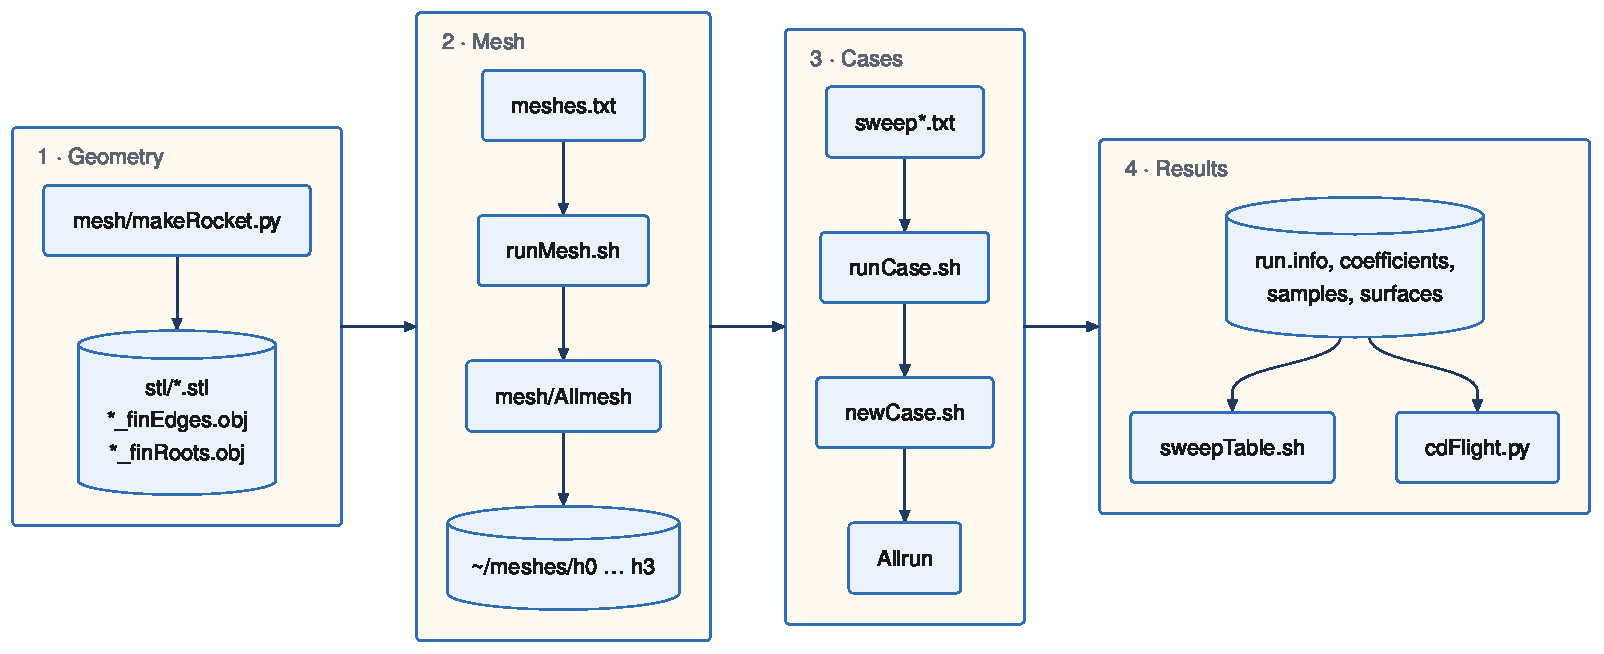
\includegraphics[width=\linewidth]{figures/pdf/process.pdf}
  \caption{Process from the geometry to the results.}
  \label{fig:process}
\end{figure}

\begin{steps}
\item \file{mesh/makeRocket.py} writes the geometry as an STL file and two edge
  files (\cref{ch:geometry}).
\item \file{mesh/Allmesh} makes one mesh. \file{runMesh.sh} makes all the meshes of
  \file{meshes.txt} (\cref{ch:mesh,sec:run-mesh}).
\item \file{newCase.sh} makes one case from a template, a mesh and a flight
  condition. \file{common/Allrun} runs it (\cref{ch:cases}). \file{runCase.sh}
  does the two steps for each line of a sweep file (\cref{ch:sweeps}).
\item Each run writes its coefficients, its samples and a record of the machine
  (\cref{ch:results}). \file{post/sweepTable.sh} collects a sweep in one table, and
  \file{flightData/cdFlight.py} compares it with the flight (\cref{ch:flight}).
\end{steps}

\section{Two solvers}

The case templates use two solvers, with the change at $M = 1$:

\begin{tabularx}{\linewidth}{@{}l l L@{}}
\toprule
Template & Solver & Use \\
\midrule
\file{case-pimple/} & \cmd{rhoPimpleFoam} & $M < 1$, and the first run of each $M > 1$ chain \\
\file{case-central/} & \cmd{rhoCentralFoam} & $M > 1$ \\
\bottomrule
\end{tabularx}

\medskip
\Cref{ch:solvers} gives the reasons and the models.

\section{Directory structure}

\begin{longtable}{@{}P{0.36\linewidth} P{0.58\linewidth}@{}}
\caption{Contents of \texttt{flightModel/}.}\label{tab:dirs}\\
\toprule
Path & Contents \\
\midrule
\endfirsthead
\toprule
Path & Contents \\
\midrule
\endhead
\file{mesh/makeRocket.py} & Writes the geometry: the STL file and its edge files (\cref{sec:makerocket}). \\
\file{mesh/stl/} & The geometry files. \file{Aconcagua_biconvex117_roll45.stl} is the default (fins at $45^\circ$). \\
\file{mesh/Allmesh} & Makes one mesh (\cref{sec:allmesh}). \\
\file{mesh/snapPlane.py} & Sets $z = 0$ on the cut of a half mesh. \\
\file{mesh/system/} & \file{meshDict}, \file{createPatchDict}, \file{createPatchDictHalf}, \file{topoSetDictHalf}, and the dictionaries that the mesh applications need. \\
\file{mesh/meshInfo} & Reference values and fin geometry of the mesh (\cref{sec:meshinfo}). \\
\file{case-central/} & Template for \cmd{rhoCentralFoam}. It also holds the files that the two templates share. \\
\file{case-pimple/} & Template for \cmd{rhoPimpleFoam}. It holds only the files that differ. \\
\file{common/Allrun}, \file{common/Allrefine}, \file{common/machineLog.py} & Scripts that \file{newCase.sh} copies into each case. \\
\file{newCase.sh} & Makes one case (\cref{sec:make-case}). \\
\file{runMesh.sh}, \file{meshes.txt} & Make the meshes of the sweep (\cref{sec:run-mesh}). \\
\file{runCase.sh}, \file{sweep*.txt} & Make and run the cases of a sweep (\cref{sec:run-sweep}). \\
\file{post/monitor.sh} & Plots a run while it runs (\cref{sec:monitor}). \\
\file{post/sweepTable.sh} & Writes a sweep as a CSV table (\cref{sec:sweeptable}). \\
\file{post/firstLayer.py} & Measures the first cell on the walls of a mesh (\cref{sec:layers}). \\
\file{flightData/} & The TeleMega data of the flight and \file{cdFlight.py} (\cref{ch:flight}). \\
\file{docs/guide/} & This guide. \\
\bottomrule
\end{longtable}

\section{Computers}\label{sec:computers}

\begin{tabularx}{\linewidth}{@{}l L L@{}}
\toprule
 & \texttt{newton} & \texttt{nemepad} \\
\midrule
CPU & 2 $\times$ Xeon E5-2660 v4, 2 sockets of 14 cores & Ryzen 7 250, 1 socket of 8 cores, 16 threads \\
Memory & ECC & \unit{28}{GB}, no ECC \\
Open MPI & 4.1 & 5.0.10 \\
Locale & \texttt{es\_ES}: \cmd{awk} writes decimal commas (\cref{sec:ts-locale}) & \texttt{en} \\
Sweep files & \file{sweepSubsonic.txt}, \file{sweepSupersonic.txt}, one on each socket & \file{*.nemepad.txt}, one file at a time \\
Status (2026-10-18) & Out of service: the memory module DIMM\_A1 stops the computer under load & In use \\
\bottomrule
\end{tabularx}

\chapter{Installation and setup}\label{ch:setup}

\section{Requirements}

\begin{longtable}{@{}P{0.24\linewidth} P{0.70\linewidth}@{}}
\caption{Requirements.}\label{tab:requirements}\\
\toprule
Item & Requirement \\
\midrule
\endfirsthead
\toprule
Item & Requirement \\
\midrule
\endhead
OpenFOAM & ESI v2412 with cfMesh (\cmd{cartesianMesh}), and its Open MPI. \\
Tools & \cmd{bash}, \cmd{rsync}, \cmd{awk}, GNU \cmd{sed}, \cmd{xz}, \cmd{/usr/bin/time}, \cmd{jinja2-cli}. \\
Python 3 & Standard library; \cmd{matplotlib} for \file{cdFlight.py}. \\
\cmd{perf} & Optional: counts the CPU cycles and the energy of each run. \\
Memory & Proportional to the number of cells. Measure \ent{maxRSSkB} of a run on the coarsest mesh (\cref{sec:runinfo}) and scale it with the number of cells before you run a finer mesh. \cmd{cartesianMesh} needs the memory of the full rocket also for a half mesh. \\
\bottomrule
\end{longtable}

\section{Prepare the shell}

Do this step in each new shell:
\begin{shell}
source /usr/lib/openfoam/openfoam2412/etc/bashrc
\end{shell}

\begin{caution}
On WSL, put the mesh and run directories on the Linux file system, not in
\file{/mnt/c}: the input and output of OpenFOAM become several times slower.
\end{caution}

\section{Prepare the computer for a study}\label{sec:prepare-computer}

The cost of a run is a measurement only if the computer runs at a known, constant
state (\cref{sec:measurement}). Before a study:

\begin{steps}
\item Fix the CPU frequency policy: the \val{performance} governor or platform
  profile. A power-saving policy lowers the clock and changes the cost.
\item Let \cmd{perf} count events: \ent{kernel.perf_event_paranoid} $\leq 1$ for the
  cycles, $\leq 0$ also for the energy. Make the setting permanent in
  \file{/etc/sysctl.d/}.
\item Prevent suspension during the study (power settings, or \cmd{systemd-inhibit}).
\item Give the memory and the CPU sufficient cooling. Above its temperature limit,
  memory refreshes more often and loses bandwidth; a CPU lowers its clock.
\item Run one case on each CPU socket, with nothing heavy beside it. Runs on one
  socket share the memory bandwidth.
\end{steps}

\section{Build this guide}\label{sec:build-guide}

The guide needs LuaLaTeX, BibTeX and the TeX Gyre fonts. The diagrams need Node.js,
the npm package \texttt{pele} and Google Chrome.

\begin{steps}
\item Go to \file{docs/guide/}.
\item If you changed a diagram in \file{figures/src/*.mmd}, render the diagrams:
\begin{shell}
npm install
make figures
\end{shell}
  Pele renders the Mermaid source to SVG; headless Chrome prints it to a vector PDF,
  because Pele sets the colours with CSS variables.
\item Compile with \cmd{make}. Commit the source, \file{figures/pdf/} and the PDF.
\end{steps}

\chapter{Geometry}\label{ch:geometry}

\section{Requirements}\label{sec:geometry-requirements}

\begin{longtable}{@{}P{0.16\linewidth} P{0.36\linewidth} P{0.40\linewidth}@{}}
\caption{Requirements for the STL file.}\label{tab:stl-req}\\
\toprule
Item & Requirement & Reason \\
\midrule
\endfirsthead
\toprule
Item & Requirement & Reason \\
\midrule
\endhead
Format & ASCII STL & A binary STL has no solid names. All the rocket then becomes one patch. \\
Solid names & \val{nosecone}, \val{body}, \val{boattail}, \val{fins} & \file{Allmesh} changes the first three to \val{cone}, \val{walls}, \val{tail}. The dictionaries and the cases use these four names. \\
Units & Metres & \file{meshDict} and \file{meshInfo} use metres. \\
Position & Nose tip at the origin, axis along $+x$ & The refinement regions, the fin region in \file{meshInfo} and the moment reference \ent{CofR (0 0 0)} use this position. \\
Edge files & \file{<name>_finEdges.obj} and \file{<name>_finRoots.obj} next to the STL & \file{Allmesh} copies them for \ent{edgeMeshRefinement} (\cref{sec:edge-refinement}). \\
\bottomrule
\end{longtable}

\subsection{Solid names that are not in the list}

\file{Allmesh} does not stop if a solid has a different name. The patch keeps the
name of the solid. \Cref{tab:bad-names} gives the effects.

\begin{longtable}{@{}P{0.32\linewidth} P{0.62\linewidth}@{}}
\caption{Effects of a solid name that is not in the list.}\label{tab:bad-names}\\
\toprule
Step & Effect \\
\midrule
\endfirsthead
\toprule
Step & Effect \\
\midrule
\endhead
\cmd{cartesianMesh}, \ent{localRefinement} & An entry without a patch gives only a warning. The patch gets no surface refinement. The cell size near the wall is then that of the volume region (\unit{50}{mm} in \ent{nearField}), not \unit{6.25}{mm}. \\
\cmd{cartesianMesh}, \ent{boundaryLayers} & The patch gets only the global layers (\cref{sec:layers}). \\
Case, \file{0.orig/} & The boundary conditions use the names \val{cone}, \val{walls}, \val{tail}, \val{fins}. A patch with a different name has no boundary condition, and the solver stops. \\
Case, \ent{forceCoeffs} & \ent{wallPatches} in \file{meshInfo} does not contain the patch. Its force is not in the coefficients. \\
\bottomrule
\end{longtable}

Before you make a mesh from a new STL file, examine the solid names:

\begin{shell}
grep -E '^ *solid ' mesh/stl/<file>.stl
\end{shell}

\section{makeRocket.py}\label{sec:makerocket}

\file{mesh/makeRocket.py} writes the geometry from its dimensions. It writes three
files: the STL file, \file{<name>_finEdges.obj} (the leading and trailing edges of
the fins) and \file{<name>_finRoots.obj} (the root of each fin). \cmd{python3
mesh/makeRocket.py -h} gives the options. A file with one \texttt{name value} on each
line can give the dimensions (\ent{--dims}).

To write the geometry of the full mesh (fins at $0^\circ$):

\begin{shell}
python3 mesh/makeRocket.py mesh/stl/Aconcagua_biconvex117.stl
\end{shell}

To write the geometry of the half mesh (fins at $45^\circ$, the default of
\file{Allmesh}):

\begin{shell}
python3 mesh/makeRocket.py mesh/stl/Aconcagua_biconvex117_roll45.stl --finRoll 45
\end{shell}

\ent{--finRoll 45} turns the fins to $45^\circ$, $135^\circ$, $225^\circ$ and
$315^\circ$. The plane $z = 0$ then passes between two fins. The STL file is always
the whole rocket: the half mesh is cut from the full mesh (\cref{sec:half-mesh}).

\begin{table}[htbp]
\centering
\caption{Parts of the Aconcagua geometry.}\label{tab:parts}
\begin{tabularx}{\linewidth}{@{}l L l@{}}
\toprule
Part & Shape & Solid name \\
\midrule
Nose & Von Kármán, \unit{0.8}{m} long & \val{nosecone} \\
Body & Cylinder, $d = \unit{0.151}{m}$ & \val{body} \\
Fins & 4 fins, biconvex section of constant thickness \unit{11.7}{mm}, edges rounded with \unit{1}{mm}, a fillet of \unit{3}{mm} all round the root & \val{fins} \\
Boattail & Cone to $d = \unit{0.110}{m}$, and the base. Shoulder and base edge rounded with \unit{3}{mm} & \val{boattail} \\
\bottomrule
\end{tabularx}
\end{table}

\subsection{Properties of the surface}

The script writes a file only if the surface is closed and all the normals point
out. The properties in \cref{tab:surface-props} come from measurements with
\cmd{cartesianMesh}. Do not change them.

\begin{longtable}{@{}P{0.40\linewidth} P{0.54\linewidth}@{}}
\caption{Properties of the surface and the measurements that set them.}\label{tab:surface-props}\\
\toprule
Property & Reason, measured with the same \file{meshDict} \\
\midrule
\endfirsthead
\toprule
Property & Reason \\
\midrule
\endhead
Nose and body + fins + boattail are two closed shells that touch on coplanar caps. The rings of the two shells are turned by half a facet. & With a sharp shoulder, one continuous hull gave 12 to 87 negative cell volumes at the shoulder. With the shoulder rounded (\ent{--shoulderRadius}, \unit{3}{mm}) the continuous hull gave 0 on $h1$. The boattail must be in the body shell, because the root fillet of the trailing edge runs \unit{3}{mm} onto the cone. \\
Body and fins are one shell: the fin root is cut into the cylinder. & With the fins as separate shells sunk into the body, the fin-body junction was not an edge of the surface. The layers of the two surfaces met at one node in the corner. \\
The leading edge, the trailing edge and the tip of the fins have a radius (\ent{--finEdgeRadius}, \unit{1}{mm}). & With sharp edges, the layers of the two fin faces met at the edge: maximum skewness 25 to 33, non-orthogonality up to $176^\circ$. With the radius: skewness 3.7, non-orthogonality $77^\circ$ to $82^\circ$. \\
A fillet of \unit{3}{mm} all round each fin root (\ent{--finRootRadius}). & Without it, the fin face and the body met at about $90^\circ$, and the fin layers and the body layers closed to one node along the root. With it, on $h1$: non-orthogonality $81.9^\circ \to 67.7^\circ$, skewness $3.58 \to 1.89$, smallest cell $2.6 \to 6.9 \times 10^{-13}$\,m\textsuperscript{3}. \\
The base edge is rounded with \unit{3}{mm} (\ent{--baseEdgeRadius}). & \\
The root trailing edge is on the shoulder (\ent{--finFromBase} = \ent{--tailLength}). & \\
44 facets around the axis (\ent{--nTheta}). & With 96 facets the continuous hull had more negative volumes. \\
\bottomrule
\end{longtable}

The edge radius is in the section parallel to the axis. Normal to the swept leading
edge ($57^\circ$), it is approximately \unit{0.5}{mm}. The section is the convex hull
of the biconvex arcs and a circle of the radius at each edge. The profile is thus a
little thicker in approximately the first \unit{80}{mm} of the chord.

\section{Use a new geometry}

\begin{steps}
\item Write the STL file with \file{makeRocket.py} (\cref{sec:makerocket}), or put
  it in \file{mesh/stl/} with its two edge files.
\item Make sure that the STL file agrees with \cref{tab:stl-req}.
\item Change the six distances of \cmd{surfaceGenerateBoundingBox} in
  \file{Allmesh} (\cref{sec:domain}).
\item Write \ent{lBody} and \ent{rBody} of the new rocket in \file{mesh/meshInfo}.
  The refinement regions scale with them (\cref{sec:object-refinements}).
\item Change the other entries of \file{mesh/meshInfo} (\cref{sec:meshinfo}).
\item Make the mesh: \cmd{mesh/Allmesh <mesh-dir> mesh/stl/<file>.stl}.
\item Remove the old meshes. \file{runMesh.sh} does not compare the geometry
  (\cref{sec:run-mesh}).
\end{steps}

\chapter{Mesh}\label{ch:mesh}

\section{Octree principle}

\cmd{cartesianMesh} (cfMesh) makes a hexahedral octree mesh from one maximum cell size,
\ent{maxCellSize}. Every other size is a refinement level $\ell$:
\[
  \Delta_\ell = \texttt{maxCellSize}\;/\;2^{\ell}.
\]
A level acts only in its patch band or its region, and adjacent cells differ by one
level at most. Two consequences follow:

\begin{itemize}
\item A wrong level changes only its own region.
\item A change of \ent{maxCellSize} alone scales every cell size of the mesh by the same
  ratio. This makes a systematic mesh series for the convergence study
  (\cref{sec:mesh-convergence-setup}).
\end{itemize}

\section{Refinement regions}\label{sec:object-refinements}

\Cref{fig:refinement} shows the nesting of the regions; each box inside another has a
finer level. File: \file{mesh/system/meshDict}. Each mesh directory keeps its own copy.

\begin{figure}[htbp]
  \centering
  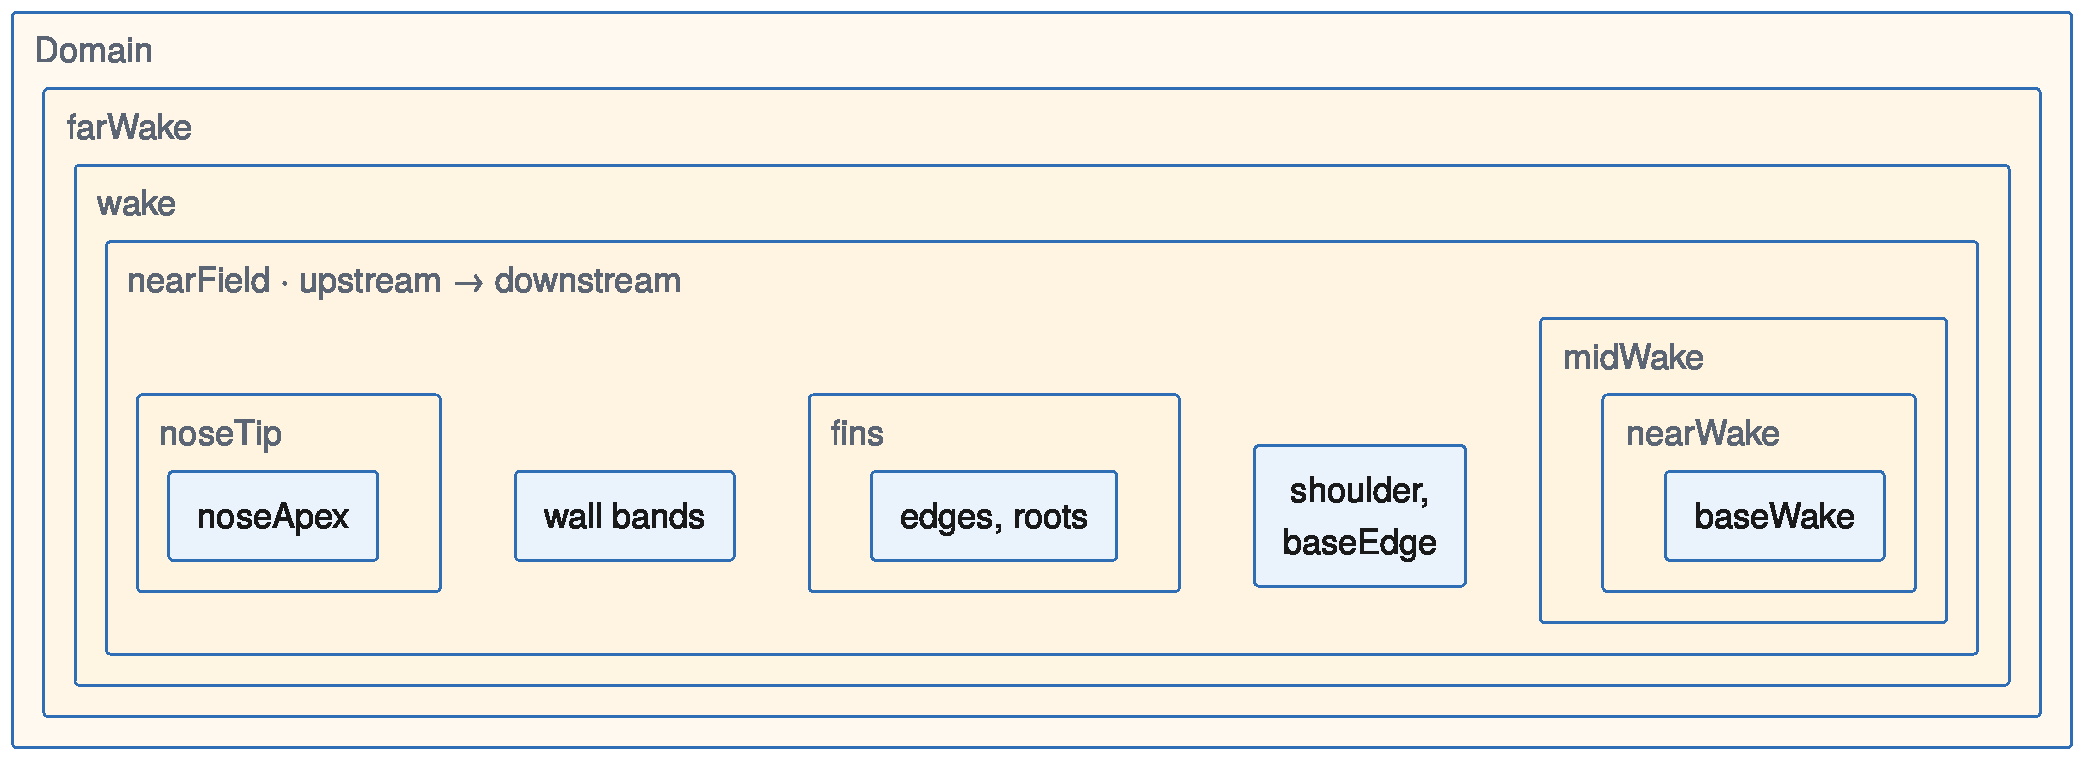
\includegraphics[width=\linewidth]{figures/pdf/refinement.pdf}
  \caption{Nesting of the refinement regions, upstream to downstream.}
  \label{fig:refinement}
\end{figure}

\begin{longtable}{@{}P{0.26\linewidth} P{0.66\linewidth}@{}}
\caption{Function of each refinement and the principle that sets its level.}\label{tab:regions}\\
\toprule
Refinement & What it resolves, and the principle \\
\midrule
\endfirsthead
\toprule
Refinement & What it resolves, and the principle \\
\midrule
\endhead
\ent{localRefinement}: \val{cone}, \val{walls}, \val{tail} & A band of thickness \ent{refinementThickness} along each wall. It contains the boundary layer and, on the nose, the region between the wall and the bow shock. The surface cell size also sets the layer thickness (\cref{sec:layers}). \\
\ent{localRefinement}: \val{fins} & The fin chord. A finer level than the body, because the fin is thin and its edges carry the strongest gradients. \\
\ent{edgeMeshRefinement}: \val{finEdges} & The leading edge (stagnation point, attached or detached shock) and the trailing edge (expansion). \\
\ent{edgeMeshRefinement}: \val{finRoots} & The fin-body junction, where the boundary layers of two walls meet. \\
\val{noseTip}, \val{noseApex} & The curvature of the nose tip: the cell must be smaller than the local radius of curvature, and the layers thinner than it. \\
\val{shoulder}, \val{baseEdge} & The expansion over the boattail and the separation at the base edge, where the base shear layer starts. They set the base pressure. \\
\val{baseWake}, \val{nearWake}, \val{midWake} & The base recirculation and the shear layer, one level coarser in each region downstream, as the wake spreads and its gradients decrease. \\
\val{nearField}, \val{wake}, \val{farWake} & Transition from the body to \ent{maxCellSize}, so that the level changes gradually. \\
\bottomrule
\end{longtable}

The regions are written as fractions of the body: each coordinate along $x$ is
multiplied by \ent{lBody}, and each coordinate across by \ent{rBody}, both from
\file{meshInfo}. The regions thus follow a rocket of another size.

The wake regions are cones on the body axis. At an angle of attack $\alpha$ the wake
moves by $\tan\alpha$ for each unit length downstream. Make sure that the wake stays
inside the wake regions over the length that sets the base pressure, for the largest
angle of the study.

\begin{caution}
\cmd{foamDictionary -set} evaluates the \texttt{\#eval} entries of \file{meshDict} and
writes numbers. \file{Allmesh} writes \ent{lBody} and \ent{rBody} with \cmd{sed}
first, for this reason. Do not set \ent{lBody} with \cmd{foamDictionary}.
\end{caution}

\section{Boundary layers}\label{sec:layers}

cfMesh extrudes the layers from the surface mesh. The thickness of the first cell
$t_1$ thus comes from the surface cell size $h$, the number of layers $n$
(\ent{nLayers}) and the growth ratio $r$ (\ent{thicknessRatio}):
\[
  t_1 \propto h\,\frac{r - 1}{r^{\,n} - 1}.
\]
\cmd{cartesianMesh} makes the layer thinner than this rule by a constant factor, so the
rule gives equal $t_1$ on meshes with equal right-hand side, but not the value of $t_1$.

\paragraph{Principle.} In a mesh study, keep $t_1$ equal on all meshes. If $t_1$
changes, \yplus{} changes, and the study mixes the change of the wall treatment with
the discretization error. As $h$ decreases from mesh to mesh, decrease $n$ or adjust
$r$ so that the rule gives the same value. \file{meshes.txt} gives $n$ and $r$ for each
mesh. Measure $t_1$ on each new mesh:
\begin{shell}
./post/firstLayer.py <mesh-dir>
\end{shell}
It gives $y$, the distance from the centre of the first cell to the wall (as
\ent{yPlus} uses it), and $t_1 = 2y$, for each wall patch, weighted by the face area.

\paragraph{Estimate of \yplus.} The mesh does not set \yplus. Estimate it before a
study from the flat-plate friction at the aft body, where \yplus{} is lowest:
\[
  Re_x = \frac{U_\infty x}{\nu_\infty},\qquad
  C_f \approx 0.0576\,Re_x^{-1/5},\qquad
  u_\tau = U_\infty\sqrt{C_f/2},\qquad
  y^+ = \frac{y\,u_\tau}{\nu}.
\]
\yplus{} grows with the speed, so one mesh gives the first cell in the viscous
sublayer at low Mach numbers and in the buffer or log layer at high Mach numbers. The
wall function of $\nu_t$ must then be valid for all \yplus{} (\cref{sec:wall-treatment}).
Measure \yplus{} on each run (\cref{sec:outputs}).

\paragraph{Layers only on wall patches.} cfMesh splits the layer only on the patches
with an entry in \ent{patchBoundaryLayers}. The global \ent{nLayers} is for the domain
faces. Keep an entry for each wall patch.

\paragraph{Fins.} The fins have fewer layers than the body
(\ent{patchBoundaryLayers/fins}). A thin fin cannot hold a thick layer stack: the
layers of the two faces meet. \ent{allowDiscontinuity} lets the number of layers change
at the fin-body junction.

\section{Domain}\label{sec:domain}

\file{Allmesh} sets the domain with \cmd{surfaceGenerateBoundingBox}, from distances to
the bounding box of the rocket. The upstream and downstream distances are fixed in
\file{Allmesh}; the lateral walls are at a fixed distance from the axis for any rocket,
so the box is symmetric about $z = 0$.

\begin{tabularx}{\linewidth}{@{}P{0.20\linewidth} L@{}}
\toprule
Boundary & Principle \\
\midrule
Upstream & In subsonic flow the disturbance of the body decays with the distance; the inlet must be far enough that the free-stream condition is correct there. In supersonic flow the inlet must be upstream of the bow shock. \\
Lateral & In subsonic flow, small blockage. In supersonic flow, the Mach cone from the nose, at the angle $\mu = \arcsin(1/M)$, exits through the lateral boundary, so that boundary needs a non-reflecting condition (\cref{sec:bc}). \\
Downstream & The outlet must be far behind the base recirculation, so that no flow enters through it. \\
\bottomrule
\end{tabularx}

\begin{caution}
\file{Allmesh} calculates the lateral distances with \cmd{awk} and sets
\cmd{LC_ALL=C}. In a locale with a decimal comma, \cmd{awk} writes numbers that
OpenFOAM reads incorrectly (\cref{sec:ts-locale}).
\end{caution}

\section{Half mesh}\label{sec:half-mesh}

If the fins have a plane of symmetry that contains the free-stream velocity, half the
domain is sufficient. By default \file{Allmesh} turns the fins so that $z = 0$ is such
a plane, meshes the whole rocket, and keeps the half $z \geq 0$:

\begin{steps}
\item The domain box is symmetric about $z = 0$, so the octree has faces on that
  plane and the cells do not cross it.
\item \cmd{topoSet} and \cmd{subsetMesh} keep the cells with the centre at $z \geq 0$.
\item \file{snapPlane.py} moves the points of the cut onto $z = 0$. The smoothing of
  \cmd{cartesianMesh} leaves them slightly off the plane.
\item \cmd{createPatch} makes the cut the patch \val{symm}, of type \val{symmetry}.
\item \file{meshInfo} gets \ent{sector half} and half the reference area, so the
  coefficients are those of the full rocket. The flow can then have an angle of
  attack in the $x$--$y$ plane, but no sideslip.
\end{steps}

\begin{caution}
Do not mesh the half domain directly, with a domain face on $z = 0$. \cmd{cartesianMesh}
treats that face as a domain boundary that touches the wall: it extrudes wall layers
into it, and the layers fan out at the corner.
\end{caution}

\section{Patches}

\cmd{createPatch} merges the six faces of the box into \val{inlet}, \val{outlet} and
\val{box}, of type \val{patch}. The \file{.fms} surface gives no type to its patches,
so \cmd{cartesianMesh} makes all of them \val{wall}; after \cmd{createPatch}, only the
rocket patches stay \val{wall}. The wall functions and the \ent{yPlus} function object
need this type. \file{Allmesh} stops if a patch in \ent{wallPatches} is not \val{wall}.

\paragraph{Feature edges.} \cmd{surfaceFeatureEdges} marks an edge as a feature edge
when the angle between the two adjacent triangles exceeds a limit. \cmd{cartesianMesh}
moves vertices onto these edges. Set the limit above the facet angle of the rounded
edges, so that only the real edges of the box and the nose are features. A low limit
marks false edges where the facets of a round are small, and the cells bend along them.

\section{meshInfo}\label{sec:meshinfo}

File: \file{mesh/meshInfo}. \file{Allmesh} copies it into the mesh directory and adds
the record of the mesh; \file{newCase.sh} copies it into the case.

\begin{longtable}{@{}P{0.28\linewidth} P{0.18\linewidth} P{0.46\linewidth}@{}}
\caption{Entries of \texttt{meshInfo}.}\label{tab:meshinfo}\\
\toprule
Entry & Written by & Function \\
\midrule
\endfirsthead
\toprule
Entry & Written by & Function \\
\midrule
\endhead
\ent{sector}, \ent{symmetryFraction} & user, \file{Allmesh} & Part of the rocket in the mesh. \file{Allrun} checks the flow angles against it. \\
\ent{Aref}, \ent{lRef} & user, \file{Allmesh} & Reference area (scaled with the sector) and length of the coefficients. \\
\ent{rBody}, \ent{lBody} & user & Scale the refinement regions. \\
\ent{fins}, \ent{finRootR}, \ent{finTipR}, \ent{finX0}, \ent{finX1} & user & Fin data for \file{Allrefine}. \\
\ent{wallPatches} & user & Patches in the force integration. \\
\ent{nCells}, \ent{maxCellSize}, \ent{finLevel}, \ent{nLayers}, \ent{thicknessRatio}, \ent{meshDir} & \file{Allmesh} & Record of the mesh. \\
\bottomrule
\end{longtable}

\section{Make a mesh}\label{sec:allmesh}

\begin{shell}
mesh/Allmesh <mesh-dir> [stl-file] [--maxCellSize <m>] [--nLayers <n>]
             [--thicknessRatio <r>] [--full]
\end{shell}

The options write into the copy of \file{meshDict}; the options that you do not give
keep the values of \file{mesh/system/meshDict}. Without \ent{--full} the mesh is a half
mesh. \file{Allmesh} does not write into a directory that exists.

\begin{figure}[htbp]
  \centering
  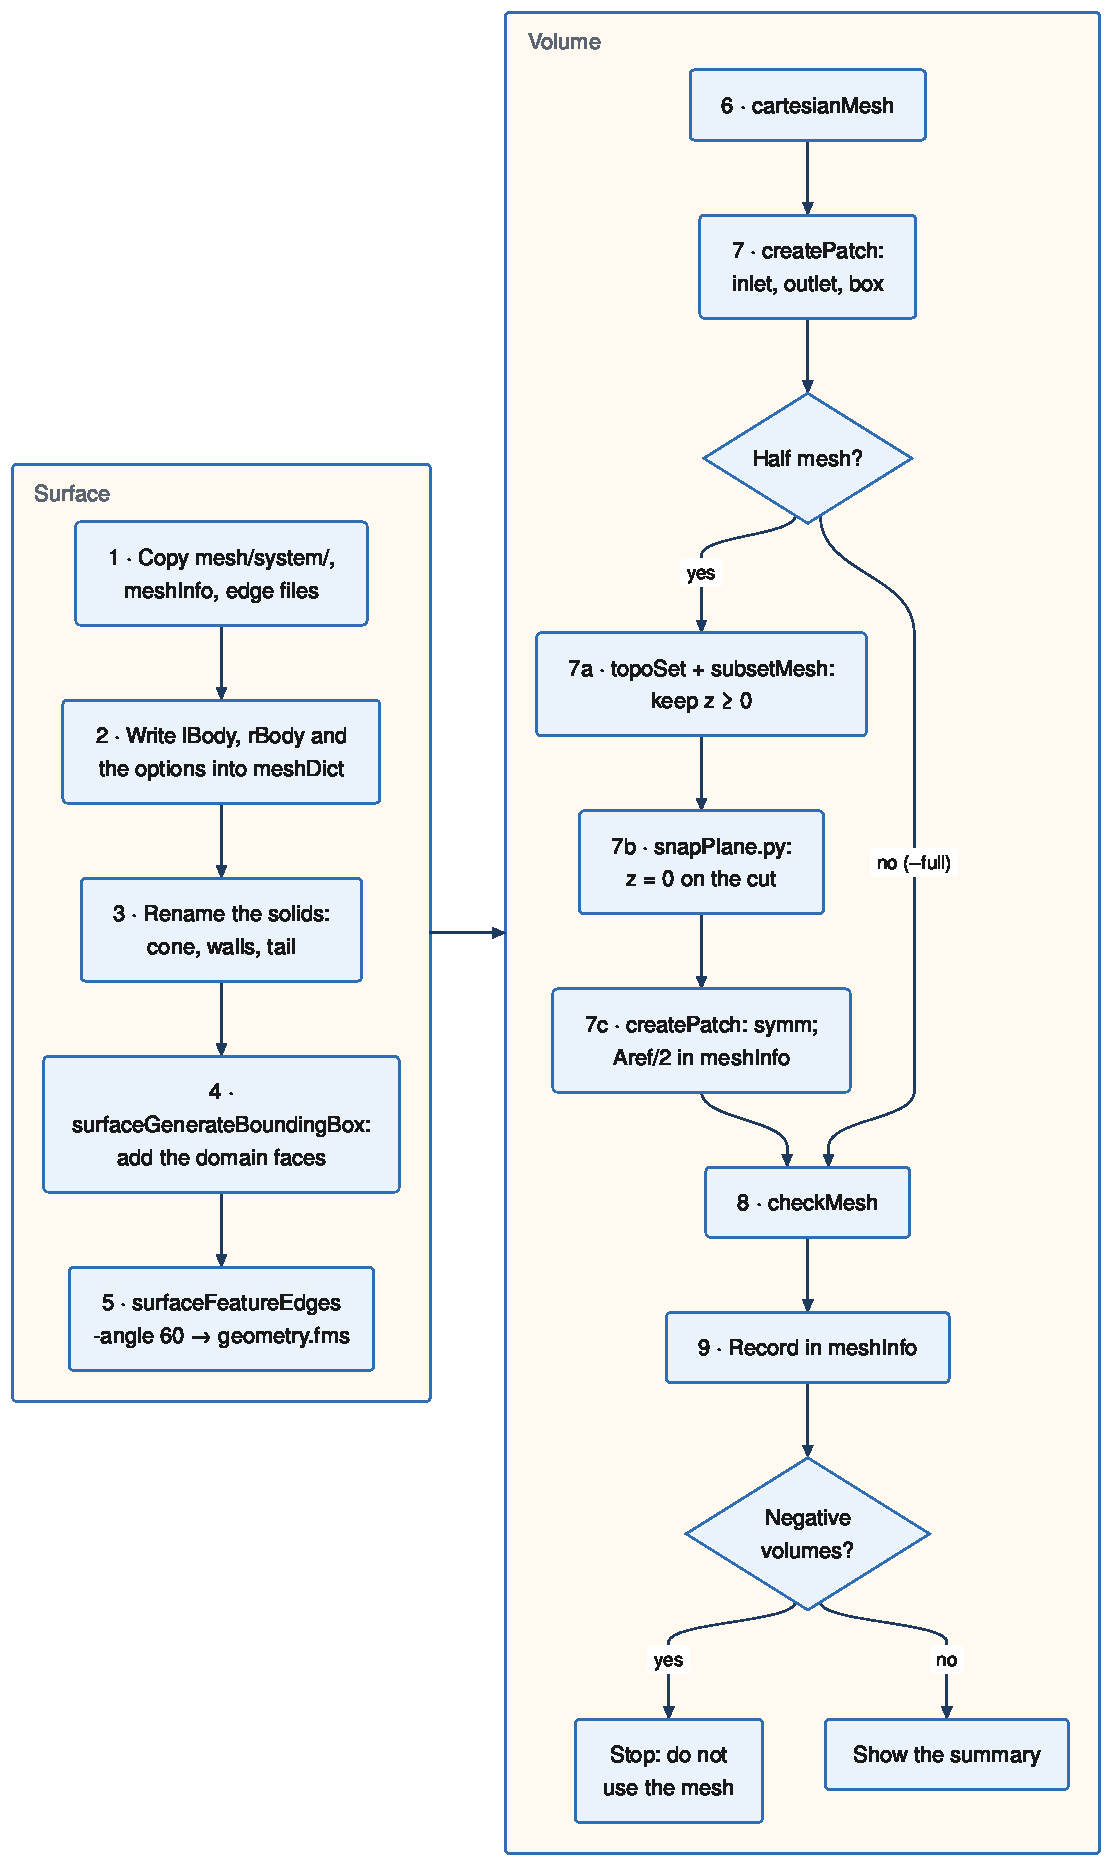
\includegraphics[width=0.85\linewidth,height=0.8\textheight,keepaspectratio]{figures/pdf/allmesh.pdf}
  \caption{Steps of \texttt{Allmesh}: surface operations, then volume operations.}
  \label{fig:allmesh}
\end{figure}

\file{Allmesh} reads the log of each application and stops on \val{FOAM FATAL}, because
\cmd{runApplication} returns 0 also when an application fails.

\section{Examine a mesh}\label{sec:examine-mesh}

\begin{steps}
\item Read the summary of \file{Allmesh}. A mesh with negative cell volumes is not
  usable: change the geometry or \file{meshDict}, and make a new mesh.
\item Examine the patch types in \file{constant/polyMesh/boundary}.
\item Measure $t_1$ with \file{post/firstLayer.py}, and compare it with the other
  meshes of the study.
\item Look at the cells on the fin edges, the base edge and the boattail shoulder in
  ParaView.
\end{steps}

\begin{note}
\cmd{checkMesh -allGeometry} also reports small determinants in layer cells, face tets
and concave cells. These checks are of a different category from negative volumes and
do not stop the use of the mesh. Record them with the mesh.
\end{note}

\chapter{Cases}\label{ch:cases}

A case is one run: one template, one mesh and one flight condition. Make it with
\file{newCase.sh} and run it with \file{Allrun}. \file{runCase.sh} does the two
steps for each line of a sweep file (\cref{ch:sweeps}).

\section{Make a case}\label{sec:make-case}

\subsection{Command}

\begin{shell}
./newCase.sh <run-dir> --mesh <mesh-dir> [options]
\end{shell}

\begin{longtable}{@{}P{0.32\linewidth} P{0.62\linewidth}@{}}
\caption{Options of \texttt{newCase.sh}.}\label{tab:newcase}\\
\toprule
Option & Function \\
\midrule
\endfirsthead
\toprule
Option & Function \\
\midrule
\endhead
\ent{--mesh <mesh-dir>} & Mandatory. The path of a mesh that \file{Allmesh} made. \\
\ent{--Minf <M>} & Free-stream Mach number. \\
\ent{--pInf <Pa>}, \ent{--Tinf <K>} & Free-stream static pressure and temperature. \\
\ent{--alpha <deg>}, \ent{--beta <deg>} & Angle of attack and angle of sideslip. \\
\ent{--Ti <->}, \ent{--nuRatio <->} & Free-stream turbulence intensity and ratio $\nu_t/\nu$. \\
\ent{--np <N>} & Number of subdomains in \file{system/decomposeParDict}. \\
\ent{--socket <S>} & Binds the run to socket \val{S}, one process per physical core (\cref{sec:binding}). \val{none} disables the binding. \\
\ent{--refine tip}, \ent{--refine fins} & Runs \file{Allrefine} on the new case (\cref{sec:refine}). \\
\ent{--init <run-dir>} & Starts from the latest time of another run (\cref{sec:init}). \\
\ent{--solver central}, \ent{--solver pimple} & Template \file{case-central/} (default) or \file{case-pimple/}. \\
\bottomrule
\end{longtable}

The flow options change entries in \file{system/flowConditions}. The options that you
do not give keep the values of the template (\cref{tab:flowconditions}).

\begin{note}
For \file{newCase.sh}, \ent{--mesh} and \ent{--init} are paths. Only
\file{runCase.sh} accepts a name without a path.
\end{note}

\subsection{Steps that newCase.sh does}

\begin{figure}[htbp]
  \centering
  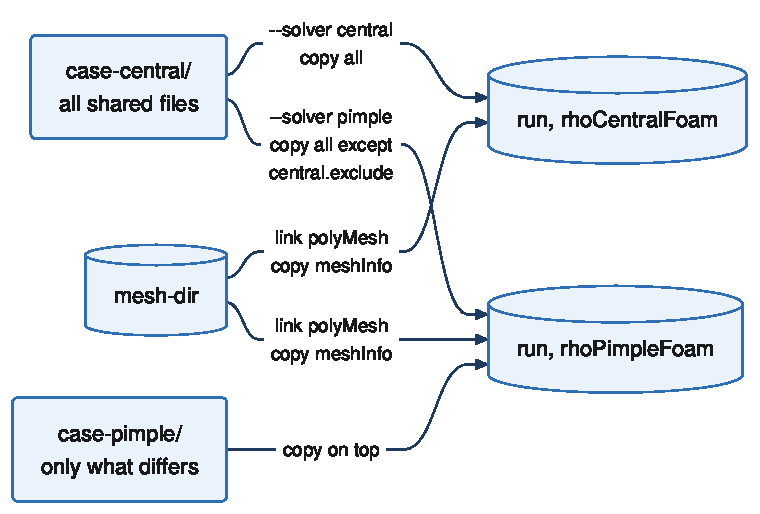
\includegraphics[width=0.75\linewidth]{figures/pdf/templates.pdf}
  \caption{How \texttt{newCase.sh} assembles a case from the templates and a mesh.}
  \label{fig:templates}
\end{figure}

\begin{steps}
\item It stops if \ent{--mesh} is missing, if the mesh has no
  \file{constant/polyMesh}, or if \file{<run-dir>} exists.
\item It copies \file{case-central/} into \file{<run-dir>}, without the mesh, the logs,
  \file{0/}, \file{processor*}, \file{postProcessing/} and the time directories. With
  \ent{--solver pimple}, it leaves out the files in \file{case-pimple/central.exclude}
  and then copies \file{case-pimple/} on top (\cref{fig:templates}).
\item It links \file{constant/polyMesh} to the mesh. With \ent{--refine} it copies it.
\item It copies \file{<mesh-dir>/meshInfo} to \file{constant/meshInfo}.
\item It copies \file{common/Allrun}, \file{common/Allrefine} and
  \file{common/machineLog.py} into the case.
\item It writes \file{run.info} with the case name, the date, the commit of the
  repository, the mesh, the number of cells and the options.
\item It renders each \file{*.j2} file with the values in \file{config.json}
  (\cref{sec:config-json}), and removes the \file{*.j2} file.
\item It writes each flow option into \file{system/flowConditions}. It stops if the
  entry does not exist.
\item It writes \ent{--np} into \file{decomposeParDict} and \ent{--socket} into the
  file \file{socket}. With \ent{--init}, it writes the path of the other run into
  \file{initFrom} and into \file{run.info}.
\item With \ent{--refine}, it runs \file{Allrefine}.
\item It adds to \file{run.info} the fingerprint of the mesh (\ent{meshHash}) and the
  physical definition of the case (block \ent{flow}, \cref{sec:nektar-same}).
\end{steps}

\section{Run a case}\label{sec:run-case}

\subsection{Command}

\begin{shell}
cd <run-dir>
./Allrun        # parallel, numberOfSubdomains from system/decomposeParDict
./Allrun 8      # parallel on 8 processes; writes 8 into decomposeParDict
./Allrun 1      # serial
\end{shell}

\subsection{Steps that Allrun does}

\Cref{fig:allrun} shows the steps.

\begin{figure}[htbp]
  \centering
  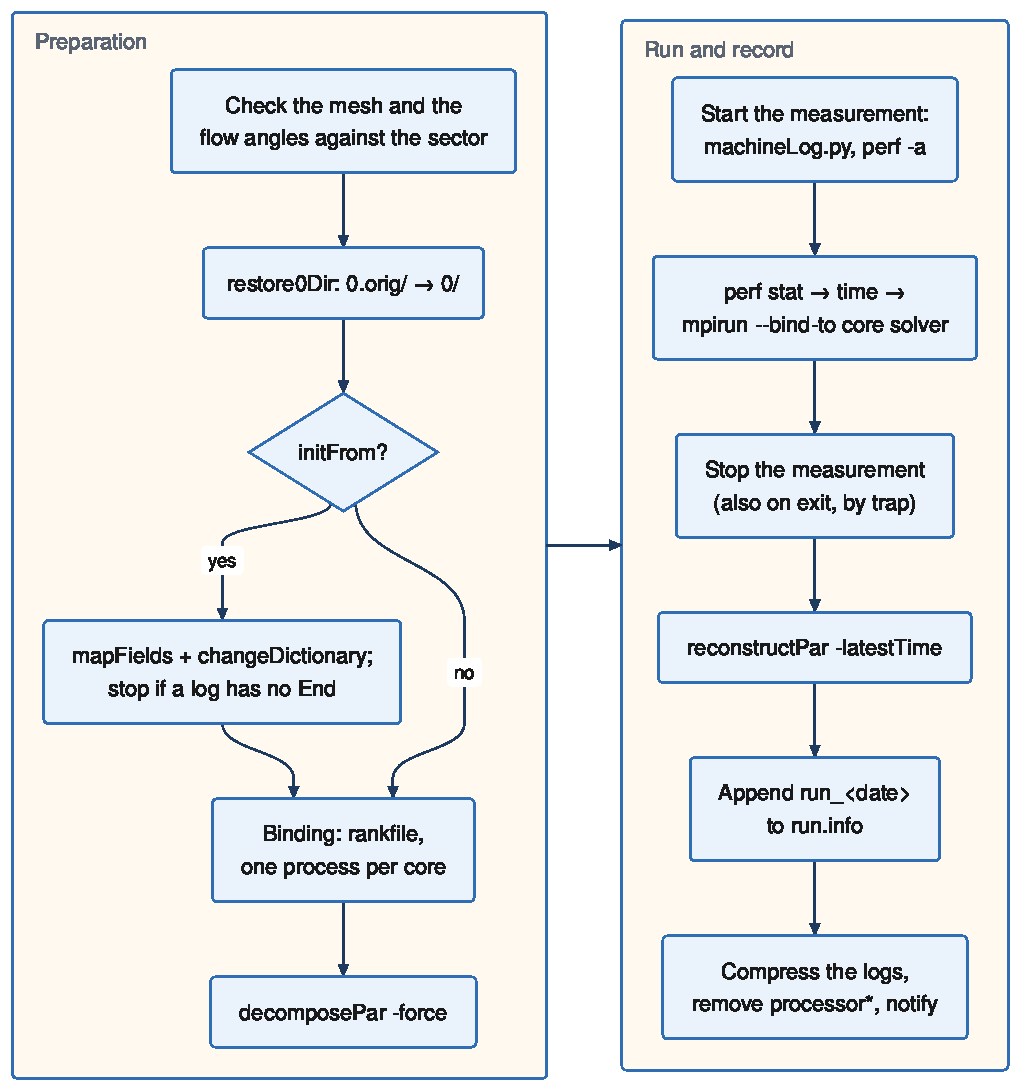
\includegraphics[width=0.9\linewidth]{figures/pdf/allrun.pdf}
  \caption{Steps of \texttt{Allrun}.}
  \label{fig:allrun}
\end{figure}

\begin{steps}
\item It stops if \file{constant/polyMesh} does not exist.
\item It compares \ent{alpha} and \ent{beta} in \file{flowConditions} with
  \ent{sector} in \file{meshInfo} (\cref{tab:sectors}). It stops if the mesh cannot
  show the flow angle.
\item It copies \file{0.orig/} to \file{0/}. If \file{initFrom} exists, it maps the
  other run onto \file{0/} (\cref{sec:init}).
\item It sets the binding of the processes (\cref{sec:binding}).
\item It runs \cmd{decomposePar -force}.
\item It starts the measurement (\cref{sec:measurement}) and runs the solver with
  \cmd{mpirun}. It stops the measurement when the solver ends. A trap also stops it
  if \file{Allrun} stops early.
\item It runs \cmd{reconstructPar -latestTime}, and removes \file{processor*} if that
  step ends correctly.
\item It adds a record \ent{run_<date>} to \file{run.info} (\cref{sec:runinfo}),
  compresses the logs with \cmd{xz} and sends the notification (\cref{sec:notify}).
\end{steps}

\begin{table}[htbp]
\centering
\caption{Flow angles that each mesh sector permits.}\label{tab:sectors}
\begin{tabular}{@{}ll@{}}
\toprule
\ent{sector} & Permitted angles \\
\midrule
\val{quarter} & $\alpha = 0$ and $\beta = 0$ \\
\val{half} & $\beta = 0$ (the default mesh) \\
\val{full} & All angles \\
\bottomrule
\end{tabular}
\end{table}

\subsection{Process binding}\label{sec:binding}

\file{Allrun} binds each MPI process to one physical core when:
\begin{itemize}
\item the case has a file \file{socket} with a socket number, or
\item the computer has one socket and the number of processes is not more than the
  number of physical cores.
\end{itemize}

It writes a \file{rankfile} with process $i$ on core $i$ of the socket, and runs
\cmd{mpirun --bind-to core}. It stops if the processes are more than the cores of the
socket. To run without binding, for example a short test beside a sweep, write
\val{none} in the file \file{socket}.

\begin{caution}
\file{Allrun} does not use the OpenFOAM function \cmd{runParallel}, because it always
adds \cmd{--oversubscribe}. With that option, Open MPI 5 ignores the
\file{rankfile}, and each process can move to all CPUs. \file{run.info} then shows a
binding that did not occur. To check the binding of a run, examine each process:
\cmd{taskset -cp <pid>} must give the two threads of one core.
\end{caution}

\subsection{End of a run}

The run stops at \ent{endTime}, or when the stop criterion finds that the mean of
$C_D$ is constant (\cref{sec:stop-criterion}). The record in \file{run.info} gives
\ent{status ok} if the solver log ends with \val{End}.

\subsection{Continue a run}

\file{controlDict} has \ent{startFrom latestTime}. Run \cmd{./Allrun} again in the same
directory to continue from the last time directory. The continuation adds a new
record to \file{run.info} and writes the function objects into a new directory with
its start time.

\begin{caution}
\file{Allrun} runs \cmd{decomposePar -force}, which removes the \file{processor*}
directories. If the solver stopped before \cmd{reconstructPar}, run
\cmd{reconstructPar -latestTime} before you run \cmd{./Allrun} again. If you do not,
you lose the data after the last reconstructed time.
\end{caution}

On the first continuation, read the start time in the solver log. Make sure that it
is the last time and not 0.

\subsection{Start a run again from zero}

\begin{steps}
\item Remove the time directories and the processor directories:
  \cmd{rm -rf [1-9]* processor*}.
\item Run \cmd{./Allrun}.
\end{steps}

\file{./Allclean} also removes \file{constant/polyMesh}. After \file{./Allclean}, make a
new case with \file{newCase.sh}.

\section{Start from another run}\label{sec:init}

\cmd{newCase.sh --init <run-dir>} starts the case from the solution of another run
instead of the uniform free stream. The sweep uses it from a coarse mesh to the next
finer mesh at the same flight condition, as the OpenFOAM ToolChain does
\citep[§5.4]{toolchain2026}. The fine mesh starts with the shock, the wake and the
boundary layer in place. The two runs can use different solvers. After
\cmd{restore0Dir}, \file{Allrun} does these steps:

\begin{steps}
\item It reads the value of each \val{fixedValue} patch in \file{0/}. These are the
  values of this run: in a supersonic case, \ent{p} on \val{inlet}.
\item It runs \cmd{mapFields <run-dir> -consistent -sourceTime latestTime}. This maps
  the internal field and the patch values. The other run can have another mesh of
  the same domain and patches.
\item It runs \cmd{changeDictionary} to write back the values of step 1.
\item It stops if the log of \cmd{mapFields} or of \cmd{changeDictionary} does not end
  with \val{End}.
\end{steps}

The free-stream entries of the patches (\ent{freestreamValue}, \ent{inletValue},
\ent{fieldInf}) are not mapped. They keep the values of this run. The other run must
have a time directory with the solution.

\begin{caution}
\cmd{mapFields} stops with a segmentation fault when it maps onto the same mesh
($h0 \to h0$), at the field \ent{Ma} (2026-10-17). The supersonic chain does this
mapping (pimple $\to$ central on $h0$). \file{Allrun} now stops the run. Before this
check, the run continued from the uniform free stream and \file{Allrun} reported the
mapping as correct. See \cref{sec:ts-mapfields}.
\end{caution}

\section{Refine the mesh near the fins (optional)}\label{sec:refine}

\begin{shell}
./Allrefine          # same as ./Allrefine tip
./Allrefine tip      # cell set finTip: a band around the fin tip
./Allrefine fins     # cell set finBox: the full fin, from root to tip
\end{shell}

Do this procedure in the case directory, before \cmd{./Allrun}, or give
\ent{--refine} to \file{newCase.sh}. \file{Allrefine} does these steps:

\begin{steps}
\item It stops if \file{0/U} exists. \cmd{refineMesh} maps the fields, so a refinement
  after a run changes the results.
\item It stops if \file{meshInfo} does not have \ent{fins true} and \ent{finTipR}.
\item It replaces the link to the mesh with a copy, so that it does not change the
  shared mesh.
\item It runs \cmd{topoSet}. \file{system/topoSetDict} makes the cell sets from the fin
  geometry in \file{meshInfo}.
\item It runs \cmd{refineMesh}. Each cell in the set becomes 8 cells.
\item It runs \cmd{checkMesh} and \cmd{renumberMesh}, and writes the new number of
  cells into \file{meshInfo}.
\end{steps}

\begin{tabularx}{\linewidth}{@{}l P{0.34\linewidth} L@{}}
\toprule
Set & Region & Effect on \yplus \\
\midrule
\val{finTip} & Annulus from $\texttt{finTipR} - \texttt{tipBand}$ to $\texttt{finTipR} + \texttt{margin}$ & None. The region does not touch the body. \\
\val{finBox} & Cylinder of radius $\texttt{finTipR} + \texttt{margin}$ & The first body cell below the fins is half as thick, so \yplus{} there is approximately half. \\
\bottomrule
\end{tabularx}

\chapter{Studies and sweeps}\label{ch:sweeps}

A study is a set of runs: flight conditions $\times$ angles of attack $\times$ meshes.
\file{runMesh.sh} makes the meshes; \file{runCase.sh} makes and runs the cases on the
meshes that exist.

\section{Design of a study}\label{sec:study-design}

\begin{tabularx}{\linewidth}{@{}P{0.22\linewidth} L@{}}
\toprule
Dimension & Principle \\
\midrule
Mach numbers & Points of the flight where the drag must be known, with more points where $C_D$ changes fast (the transonic rise). \\
Flight conditions & $p_\infty$ and $T_\infty$ of the real atmosphere at the height where the vehicle passed each Mach number, so that the Reynolds number is that of the flight (\cref{sec:flight-conditions}). \\
Angles of attack & From zero to the largest angle that the flight reached, with margin. Measure the flight angle when possible (\cref{sec:flight-alpha}). \\
Meshes & At least three meshes of one systematic series for the error estimate, plus a coarser mesh to start the runs (\cref{sec:mesh-convergence-setup}). \\
\bottomrule
\end{tabularx}

\subsection{Chains of runs}

Each flight condition and angle is a chain: each run starts from the solution on the
coarser mesh (\ent{--init}, \cref{sec:init}). The fine mesh then starts with the
shocks, the wake and the boundary layer in place, and skips the start transient, which
is the most expensive and least stable part of a run \citep[§5.4]{toolchain2026}.

\begin{figure}[htbp]
  \centering
  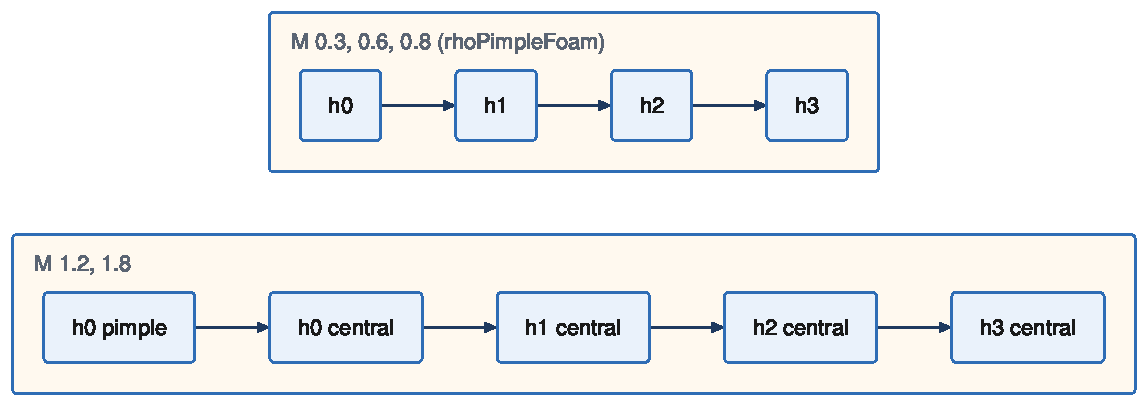
\includegraphics[width=0.95\linewidth]{figures/pdf/chains.pdf}
  \caption{Chains of runs. Left to right: from coarse to fine. Each arrow is an \texttt{--init}.}
  \label{fig:chains}
\end{figure}

A supersonic chain starts with a \cmd{rhoPimpleFoam} run on the coarsest mesh, because
\cmd{rhoCentralFoam} from a uniform free stream fails at the base
(\cref{sec:supersonic-start}).

\subsection{Mesh series for the convergence study}\label{sec:mesh-convergence-setup}

\begin{steps}
\item Change only \ent{maxCellSize}, with a constant ratio, and keep all levels. All
  cell sizes then change by the same ratio.
\item Use a ratio that gives a refinement ratio of more than 1.3 in the representative
  cell size, as the method of \citet{celik2008} needs. An octree mesh does not refine
  uniformly: calculate the real ratio of each pair from the number of cells,
  $r = (N_\text{fine}/N_\text{coarse})^{1/3}$, and use it in \cref{sec:gci}.
\item Keep $t_1$ equal on all meshes (\cref{sec:layers}).
\item Run the same flight conditions on all meshes.
\end{steps}

\section{Make the meshes}\label{sec:run-mesh}

\file{meshes.txt} has one mesh on each line: a name, then the options of
\file{Allmesh}. Lines that start with \texttt{\#} have no effect.

\begin{shell}
./runMesh.sh [meshes-file] [meshes-dir]      # default: meshes.txt, ~/meshes
\end{shell}

For each line: if the mesh exists with the same options, \file{runMesh.sh} keeps it; if
the options differ, it stops; if not, it runs \file{Allmesh}. It does not compare the
geometry: after a change of the STL file, remove the old meshes. To make one mesh only,
give a file with that line.

\section{Run the cases}\label{sec:run-sweep}

A sweep file has one case on each line: a name, then the options of \file{newCase.sh}
(\cref{tab:newcase}). A mesh or an \ent{--init} without \texttt{/} is a name in
\file{<meshes-dir>} or \file{<runs-dir>}. The run of an \ent{--init} must come earlier
in the file.

\begin{shell}
m08-a00-h1  --mesh h1 --solver pimple --alpha 0 --Minf 0.8 --pInf <Pa> --Tinf <K> --init m08-a00-h0
\end{shell}

\begin{shell}
./runCase.sh [--np <N>] [--socket <S>] <sweep-file> [runs-dir] [meshes-dir]
\end{shell}

The defaults are the physical cores of one socket, \file{~/runs} and \file{~/meshes}.
The sweep files do not contain the number of processes, so the same file works on any
computer. An option on a line of the file overrides the option of \file{runCase.sh}.

For each line, \file{runCase.sh} skips the case if its directory exists, stops if the
mesh does not exist, runs \file{newCase.sh}, and runs \file{Allrun}. A failed run does
not stop the sweep. Thus, after a stop, run \file{runCase.sh} again: it continues from
the first case that does not exist.

\paragraph{Processes and sockets.} One process for each physical core of one socket,
bound to its core (\cref{sec:binding}), is the default. On a computer with two sockets,
run \file{sweepSubsonic.txt} with \ent{--socket 0} and \file{sweepSupersonic.txt} with
\ent{--socket 1} at the same time. Each chain must stay in one file, because the files
run in parallel.

\subsection{Start a sweep}

\begin{steps}
\item Do the steps of \cref{sec:prepare-computer}.
\item Start the sweep so that it continues when the terminal closes:
\begin{shell}
nohup ./runCase.sh <sweep-file> > ~/log.<sweep> 2>&1 &
\end{shell}
\item On the first case, examine the binding (\cref{sec:binding}) and the measurement
  files (\cref{sec:measurement}).
\end{steps}

\subsection{Stop a sweep}

\begin{steps}
\item Stop \file{runCase.sh} by its process number (\cmd{kill <pid>}). No new case
  starts; the current solver continues.
\item To stop the solver also, stop its \cmd{mpirun} (or \cmd{prterun}) by its process
  number. \file{Allrun} then reconstructs the last time, writes the record and stops
  the measurement.
\end{steps}

\begin{caution}
\file{runCase.sh} reads the sweep file while it runs. Do not edit the file in place
until the sweep stops.
\end{caution}

\section{Flight conditions}\label{sec:flight-conditions}

The conditions of each Mach number come from the flight telemetry
(\cref{ch:flight}): the ambient pressure and temperature at the height where the vehicle
passed that Mach number in the coast phase, with the atmosphere of the day of the
flight. The standard atmosphere can differ by tens of kelvin from the real one, which
changes the Mach number at a given speed, the density and the Reynolds number.
\file{cdFlight.py} prints the conditions; write them into the sweep files.

\section{Rules}

\begin{itemize}
\item Do not put meshes or runs in the repository. Put the STL file, \file{meshDict},
  \file{meshes.txt} and the sweep files in it.
\item When a change to \file{meshDict} changes the mesh, commit it with the
  \cmd{checkMesh} summary of the new mesh.
\end{itemize}

\chapter{Solvers and models}\label{ch:solvers}

This chapter gives the principle behind each choice of the templates and the file
where each value is. Read the values in the files.

\section{Two solvers}\label{sec:two-solvers}

\begin{tabularx}{\linewidth}{@{}P{0.20\linewidth} L L@{}}
\toprule
 & \file{case-pimple/}: \cmd{rhoPimpleFoam} & \file{case-central/}: \cmd{rhoCentralFoam} \\
\midrule
Formulation & Pressure-based, \ent{transonic} pressure equation & Density-based, explicit, central-upwind flux \\
Use & $M < 1$; start of each $M > 1$ chain & $M > 1$ \\
\bottomrule
\end{tabularx}

\medskip
The numerical dissipation of a central-upwind flux scales with the speed of sound, not
with the flow speed. At low Mach numbers it is thus large compared with the convective
flux, and the drag error grows. A pressure-based solver does not have this problem, but
it loses accuracy where strong shocks occur. The OpenFOAM ToolChain report
\citep[§6]{toolchain2026} measured both effects on rockets. The workflow therefore
changes solver at $M = 1$.

\begin{caution}
The change of discretization at $M = 1$ can cause a step in $C_D(M)$ that is not
physical. To measure it, run one Mach number with both solvers on the same mesh.
\end{caution}

The models, the gas, the boundary conditions, the function objects and the flight
condition are the same files in the two templates: \file{case-pimple/} holds only the
files that differ (\cref{sec:pimple}).

\section{Files of the templates}

\begin{longtable}{@{}P{0.40\linewidth} P{0.52\linewidth}@{}}
\caption{Files of the templates and their function.}\label{tab:template-files}\\
\toprule
File & Function \\
\midrule
\endfirsthead
\toprule
File & Function \\
\midrule
\endhead
\file{system/flowConditions} & The flight condition: the only input of a case (\cref{sec:flow-conditions}). \\
\file{system/flowDerived} & Values derived from \file{flowConditions} with \texttt{\#eval}. \\
\file{config.json} & Courant ramp and stop criterion; \file{newCase.sh} renders the \file{*.j2} files with it. \\
\file{0.orig/} & Boundary and initial conditions (\cref{sec:bc}). \\
\file{constant/thermophysicalProperties} & Gas model (\cref{sec:thermo}). \\
\file{constant/turbulenceProperties} & Turbulence model (\cref{sec:turbulence}). \\
\file{system/controlDictBase.j2}, \file{FOs/FOcommon} & Time control and function objects (\cref{sec:function-objects}). \\
\file{system/fileUpdater.j2}, \file{fileUpdaterControlDict/} & The Courant ramp of the central template (\cref{sec:ramp}). \\
\file{system/FOs/FOrunTimeControl.j2} & Stop criterion (\cref{sec:stop-criterion}). \\
\file{system/fvSchemes*}, \file{system/fvSolution} & Schemes and linear solvers (\cref{sec:schemes}). \\
\bottomrule
\end{longtable}

\begin{caution}
Use \cmd{foamDictionary -set} only on \file{flowConditions}. On a file with
\texttt{\#include} or \texttt{\#eval}, it writes the expanded values, and the file stops
following \file{flowConditions}.
\end{caution}

\section{Flight condition}\label{sec:flow-conditions}

\file{flowConditions} holds $M_\infty$, $p_\infty$, $T_\infty$, $\alpha$, $\beta$, the
turbulence intensity $T_i$ and the ratio $\nu_t/\nu$ of the free stream.
\file{flowDerived} calculates from them:
\[
  a_\infty = \sqrt{\gamma R T_\infty},\quad
  U_\infty = M_\infty a_\infty,\quad
  \rho_\infty = \frac{p_\infty}{R T_\infty},\quad
  \mu_\infty = \frac{A_s\sqrt{T_\infty}}{1 + T_s/T_\infty},
\]
\[
  k_\infty = \tfrac32 (U_\infty T_i)^2,\quad
  \nu_{t\infty} = \frac{\nu_t}{\nu}\,\nu_\infty,\quad
  \omega_\infty = \frac{k_\infty}{\nu_{t\infty}},
\]
and the velocity, drag and lift directions from $\alpha$ and $\beta$ (wind axes). The
free-stream turbulence is small and the eddy-viscosity ratio of order one, so that the
free stream does not change the boundary layer.

\section{Numerical method of rhoCentralFoam}

\cmd{rhoCentralFoam} advances the conserved variables $\rho$, $\rho\mathbf{U}$ and
$\rho E$ explicitly, then corrects the diffusive terms implicitly. It solves no
pressure equation.

\paragraph{Flux.} The central-upwind scheme of Kurganov
\citep{kurganov2000,kurganov2001} weights the face flux with the local one-sided wave
speeds. It captures shocks without a Riemann solver and without artificial viscosity.
\citet{greenshields2010} give its implementation in OpenFOAM.

\paragraph{Reconstruction.} The primitive variables go to the faces with the van Leer
TVD limiter \citep{vanleer1979}: second order in smooth regions, first order at a
discontinuity, so no new extrema occur at shocks.

\section{Local time step, Courant ramp and stop criterion}

\subsection{Local time step}\label{sec:lts}

The templates solve a steady problem with a pseudo-transient march (\ent{ddt
localEuler}). Each cell advances with the largest time step that its own Courant number
permits. The intermediate states are not physical; the converged state is. The cost
then depends on the number of iterations, not on the smallest cell of the mesh, which
with a global step sets the step of the whole domain.

\ent{deltaT} is 1, so the time counts iterations: \ent{endTime}, the write interval,
the ramp and the stop criterion are in iterations. The central template reads the
local-step controls in \file{controlDict}, the pimple template in the \ent{PIMPLE}
dictionary of \file{fvSolution}.

\begin{caution}
With \ent{localEuler}, the Courant number that \cmd{rhoCentralFoam} writes uses the
global \ent{deltaT}, not the local step: it is meaningless. Read the line
\val{Flow time scale min/max}: its minimum is the step of the most restrictive cell, and
a sudden decrease shows a cell that diverges.
\end{caution}

\subsection{Courant ramp (central template)}\label{sec:ramp}

A uniform free stream on a no-slip wall is a strong impulsive start. The explicit
central solver has no damping of the local step, so a large Courant number at the
start makes the solution leave the physical range. The ramp \citep[§5.4.1]{toolchain2026}
starts with a small Courant number and first-order reconstruction, increases the
Courant number step by step, then changes to second order and ramps again
(\cref{fig:ramp}). The function objects \ent{timeActivatedFileUpdate} copy a new
\file{controlDict} or \file{fvSchemes} at each switch; \ent{runTimeModifiable} makes the
solver read it.

\begin{figure}[htbp]
  \centering
  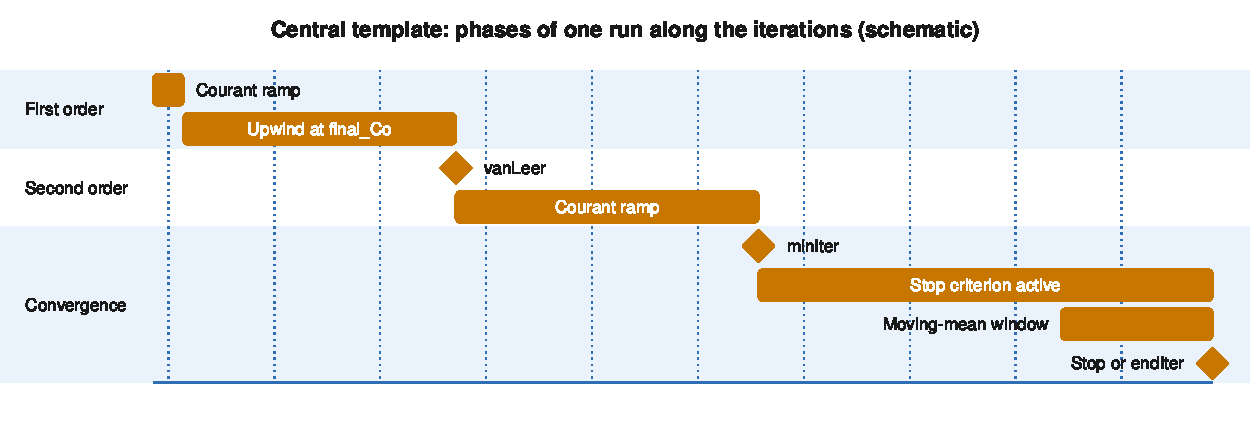
\includegraphics[width=\linewidth]{figures/pdf/ramp.pdf}
  \caption{Phases of a run of the central template along the iterations. The diamonds are the keys of \texttt{config.json} that place each switch.}
  \label{fig:ramp}
\end{figure}

The final Courant number never comes before the end of the ramp: a jump of the Courant
number makes the explicit solver fail some iterations later. The pimple template has
no ramp: its implicit pressure-velocity coupling damps the start.

\subsection{config.json}\label{sec:config-json}

\begin{tabularx}{\linewidth}{@{}P{0.26\linewidth} L@{}}
\toprule
Key & Function \\
\midrule
\ent{maxCo} (pimple), \ent{final_Co} (central) & Courant number of the converged phase. \\
\ent{vanLeer} (central) & Iteration of the change from first to second order. \\
\ent{minIter} & First iteration of the stop criterion. In the central template, also the change to the final Courant number. \\
\ent{endIter} & Last iteration if the criterion does not stop the run. \\
\ent{coeffs_fields}, \ent{coeffs_variation}, \ent{coeffs_window} & Coefficients, absolute tolerances and window of the stop criterion. \\
\bottomrule
\end{tabularx}

\medskip
The schedule comes from the ToolChain, which used another rocket. Adjust it from the
first runs: the iteration at which $C_D$ becomes flat in first order, and the
iterations that the second order needs.

\subsection{Stop criterion}\label{sec:stop-criterion}

For each coefficient $C$ in \ent{coeffs_fields}, \ent{runTimeControl} calculates the
moving mean $\overline{C}$ over \ent{coeffs_window} iterations, from \ent{minIter}. The
run stops when the window is complete and
\[
  |\overline{C} - C| < \texttt{coeffs\_variation}
\]
for all coefficients. Set the tolerance as a fraction of the expected coefficient: an
absolute tolerance is a smaller fraction of a large coefficient. The tolerance is
absolute, so it also works for a coefficient near zero, such as $C_L$ at $\alpha = 0$.
At $\alpha \neq 0$, add $C_L$ and $C_m$ to the criterion, or examine that they are flat.

To change the tolerance of a running case, edit \ent{tolerance} in its
\file{system/FOs/FOrunTimeControl} and \cmd{touch system/controlDict}. The mean then
starts again from zero.

\section{Turbulence}\label{sec:turbulence}

RANS with the $k$--$\omega$ SST model \citep{menter1994}, in the version of
\citet{menter2003} that OpenFOAM uses. The Boussinesq hypothesis gives the Reynolds
stress from an eddy viscosity,
\[
  -\overline{u_i'u_j'} = \nu_t\left(\frac{\partial U_i}{\partial x_j} + \frac{\partial U_j}{\partial x_i}\right) - \tfrac23 k\,\delta_{ij},
  \qquad
  \nu_t = \frac{a_1 k}{\max(a_1\omega,\ S F_2)}.
\]
The shear-stress limiter in the denominator limits $\nu_t$ in adverse pressure
gradients, which occur on the boattail and at the fin-body junction and set the base
flow. When you compare with the literature, find which SST version the source uses.

\subsection{Wall treatment}\label{sec:wall-treatment}

\begin{tabularx}{\linewidth}{@{}l P{0.34\linewidth} L@{}}
\toprule
Field & Condition & Principle \\
\midrule
\ent{nut} & \ent{nutUSpaldingWallFunction} & Spalding's law \citep{spalding1961} is one formula from the viscous sublayer through the buffer layer to the log layer, so it is valid for any \yplus{} of the first cell. \\
\ent{k} & \ent{kLowReWallFunction} & Also continuous in \yplus. \\
\ent{omega} & \ent{omegaWallFunction} & Blends the sublayer and log-layer values. \\
\ent{alphat} & \ent{compressible::alphatWallFunction} & Turbulent heat diffusivity from $\nu_t$ and $Pr_t$. \\
\bottomrule
\end{tabularx}

\medskip
A \yplus-insensitive wall treatment is necessary, because one mesh gives different
\yplus{} at different Mach numbers (\cref{sec:layers}). The conditions need wall
patches of type \val{wall}.

\section{Gas}\label{sec:thermo}

Air as a perfect gas ($p = \rho R T$) with constant $c_p$ (\val{hConst}), energy as
sensible internal energy, and Sutherland viscosity, $\mu = A_s\sqrt{T}/(1 + T_s/T)$
\citep[eq.~1-36]{white2006}. \cmd{rhoCentralFoam} needs \val{hePsiThermo} and the
internal energy.

\paragraph{Prandtl number.} With Sutherland transport, OpenFOAM calculates the
conductivity with the modified Eucken correction,
$\kappa = \mu\,c_v\,(1.32 + 1.77\,R/c_v)$. The laminar Prandtl number is therefore an
output, not an input:
\[
  Pr = \frac{c_p}{c_v\,(1.32 + 1.77\,R/c_v)}.
\]
For air it is lower than the usual 0.72. Another solver must use the same value
(\cref{ch:nektar}). The turbulent Prandtl number $Pr_t$ is an input \citep{kays1994}.

\paragraph{Validity of constant $c_p$.} The stagnation temperature is
$T_0 = T\,(1 + \tfrac{\gamma-1}{2}M^2)$. When $T_0$ is high enough that $c_p$ of air
changes by more than the accepted error, replace \val{hConst} with \val{janaf}. The
\cmd{rhoCentralFoam} tutorial \file{biconic25-55Run35} has the air coefficients.

\paragraph{Gas constant.} \file{flowDerived} and the thermophysical model must use the
same $R$, $\gamma$ and Sutherland constants. Compare them when you change one.

\section{Boundary conditions}\label{sec:bc}

The number of characteristics that enter the domain through a boundary sets the number
of values that the boundary may impose.

\begin{tabularx}{\linewidth}{@{}l P{0.30\linewidth} L@{}}
\toprule
Field & \val{inlet}, \val{outlet}, \val{box} & Principle \\
\midrule
\ent{U} & \val{freestreamVelocity} & Fixed where the flow enters, extrapolated where it leaves. \\
\ent{T}, \ent{k}, \ent{omega} & \val{inletOutlet} & The same. \\
\ent{p}, $M < 1$ & \val{freestreamPressure} & One acoustic wave enters through the outlet, so $p$ is fixed where the flow leaves and extrapolated where it enters. \\
\ent{p}, $M > 1$ & \val{fixedValue} inlet, \val{zeroGradient} outlet, \val{waveTransmissive} box & All characteristics enter at a supersonic inlet and leave at a supersonic outlet. On the lateral boundary the Mach cone leaves the domain: a non-reflecting condition \citep{poinsot1992} prevents its reflection. \\
\bottomrule
\end{tabularx}

\medskip
\file{0.orig/p} selects the branch with \texttt{\#if} on \ent{Minf}, because
\val{freestreamPressure} has no supersonic mode in v2412.

\paragraph{Walls.} No slip and adiabatic (\val{zeroGradient} on $T$). During a short
motor burn, the airframe does not get near the recovery temperature, so zero heat flux
is the correct limit.

\section{Function objects}\label{sec:function-objects}

\file{system/FOs/FOcommon} is common to the two templates. \Cref{ch:results} lists
the outputs. The force coefficients use the density field (the pressure is in Pa), the
free-stream density and speed for the dynamic pressure, \ent{Aref} and \ent{lRef} from
\file{meshInfo}, the nose tip as the moment reference, and the wind axes.

\section{Discretization schemes and linear solvers}\label{sec:schemes}

\begin{tabularx}{\linewidth}{@{}P{0.34\linewidth} L@{}}
\toprule
Choice & Principle \\
\midrule
TVD limiters on the convection of the flow variables & Second order without new extrema at shocks. \\
First-order upwind for $k$ and $\omega$ & Keeps them positive. \\
Limited non-orthogonal correction & The layer cells are non-orthogonal; the limit keeps the correction bounded. \\
\ent{meshWave} wall distance & Needed by the SST blending functions. \\
\val{diagonal} for $\rho$, $\rho\mathbf{U}$, $\rho E$ (central) & The conserved variables are explicit. \\
Smooth solvers for $\mathbf{U}$, $e$, $k$, $\omega$; GAMG for $p$ (pimple) & An elliptic pressure equation needs a multigrid solver. \\
\bottomrule
\end{tabularx}

\medskip
In the central template, \file{fvSchemes} and \file{fvSchemesUpwind} include
\file{fvSchemesVanLeer} and set the reconstruction to upwind; the ramp copies them.
Do not edit \file{system/fvSchemes}.

\section{rhoPimpleFoam template}\label{sec:pimple}

\file{case-pimple/} holds \file{config.json}, \file{controlDict.j2},
\file{fvSchemes}, \file{fvSolution.j2}, \file{fvOptions} and \file{central.exclude}.
The schemes come from the transonic template of the ToolChain.

\begin{tabularx}{\linewidth}{@{}P{0.34\linewidth} L@{}}
\toprule
Choice & Principle \\
\midrule
\ent{transonic yes} & A density-weighted pressure equation for the compressibility of high subsonic flow. \\
One outer corrector & A pseudo-steady march needs one pressure-velocity pass for each iteration. \\
Bounded gradients and TVD convection & Second order away from the local shocks of transonic flow. \\
\ent{pMinFactor}, \ent{pMaxFactor} & Limits of $p$ relative to the boundary values; the upper limit must contain the stagnation pressure. \\
\ent{limitTemperature} in \file{fvOptions} & Protects the start transient. Count the limited cells in the log: after the start there must be none. \\
\bottomrule
\end{tabularx}

\section{Start of the supersonic cases}\label{sec:supersonic-start}

From a uniform free stream, the flow behind the base starts at the free-stream speed:
the base acts as a piston and empties the region behind it. The pressure and the
temperature there fall towards zero before the wake fills. The pimple template has a
temperature limit and survives this transient. \cmd{rhoCentralFoam} reads no
\file{fvOptions} in v2412, has no such limit, and fails with a floating point
exception in the thermophysical model. Therefore each supersonic chain starts with a
pimple run on the coarsest mesh, and the central run starts from it (\cref{fig:mach}).

\chapter{Results and measurement}\label{ch:results}

Each run records its coefficients, its samples, its cost and the state of the
computer in small files. A run thus can be compared with another solver without the
fields of gigabytes.

\section{Outputs of a run}\label{sec:outputs}

\begin{longtable}{@{}P{0.46\linewidth} P{0.48\linewidth}@{}}
\caption{Outputs of a run. \texttt{<t0>} is the start time: 0 for a new run.}\label{tab:outputs}\\
\toprule
File & Contents \\
\midrule
\endfirsthead
\toprule
File & Contents \\
\midrule
\endhead
\file{postProcessing/forceCoeffs1/<t0>/coefficient.dat} & $C_D$, $C_L$, \val{CmPitch}, \val{CmRoll}, \val{CmYaw}, $C_s$, each also split into front \val{(f)} and rear \val{(r)}. Every 50 steps. \\
\file{postProcessing/forces1/<t0>/force.dat}, \file{moment.dat} & Force in N and moment in N\,m: total, pressure and viscous. Every 50 steps. \\
\file{postProcessing/residuals/<t0>/solverInfo.dat} & Initial residuals. Every 50 steps. \\
\file{postProcessing/yPlus/<t0>/yPlus.dat} & \yplus{} minimum, maximum and mean for each wall patch, at each write time. \\
\file{postProcessing/timeInfo/<t0>/timeInfo.dat} & CPU and wall time, total and for the last 50 steps. \\
\file{postProcessing/surfaces/<t>/} & VTK of the skin and the symmetry plane, at the end. \\
\file{postProcessing/samples/<t>/*.csv} & Lines and points for the comparison with another solver, at the end (\cref{tab:samples}). \\
Last time directory & \ent{p}, \ent{T}, \ent{U}, \ent{rho}, \ent{k}, \ent{omega}, \ent{nut}, \ent{alphat}, \ent{Ma}, \ent{static(p)_coeff} ($C_p$), \ent{yPlus}, \ent{wallShearStress}. \\
\file{run.info} & Record of the case and of each execution (\cref{sec:runinfo}). \\
\file{log.<app>.<date>.xz} & Compressed logs. Read them with \cmd{xzless} or \cmd{xzgrep}. \\
\file{log.perf.<date>.xz}, \file{log.energy.<date>.xz}, \file{log.machine.<date>} & Measurement of the computer (\cref{sec:measurement}). \\
\bottomrule
\end{longtable}

Open the fields in ParaView with \cmd{paraview case.foam}. These quantities are not
written, but \cmd{postProcess} calculates them from the last time without a new run:

\begin{tabularx}{\linewidth}{@{}P{0.34\linewidth} L@{}}
\toprule
Quantity & Command \\
\midrule
Vorticity, Q criterion & \cmd{postProcess -func vorticity -latestTime}, \cmd{-func Q} \\
Total pressure and temperature & function object \ent{pressure} with \ent{mode total}; $T_0 = T\,(1 + \tfrac{\gamma-1}{2}M^2)$ \\
\bottomrule
\end{tabularx}

\begin{table}[htbp]
\centering
\caption{Samples for the comparison with another solver (function object \texttt{samples}).}\label{tab:samples}
\begin{tabularx}{\linewidth}{@{}l L@{}}
\toprule
Set & Contents \\
\midrule
\val{skinZ0} & The wall cut \unit{0.5}{mm} off the plane $z = 0$. Columns $x$, $y$, $z$: windward is $y < 0$, leeward is $y > 0$. \\
\val{skinY0} & The wall cut \unit{0.5}{mm} off the plane $y = 0$ (the side). The two planes pass between the fins. \\
\val{wake05}, \val{wake1}, \val{wake2}, \val{wake5} & Lines in $y$ from $-0.6$ to \unit{0.6}{m} on $z = 0$, at 0.5, 1, 2 and 5 diameters behind the base. \\
\val{axis} & From $x = \unit{-0.5}{m}$ to 20 diameters behind the base. \\
\val{freeStream} & One point \unit{1}{m} in front of the nose tip. \\
\bottomrule
\end{tabularx}
\end{table}

The samples contain $p$, $T$, $U$, $\rho$, $M$, $k$, $\omega$, $\nu_t$, $C_p$, $\tau_w$ and
\yplus, with \ent{cellPoint} interpolation.

\section{run.info}\label{sec:runinfo}

\file{newCase.sh} makes \file{run.info}. \file{Allrun} adds a record
\ent{run_<date>} each time that it runs. The file is an OpenFOAM dictionary: read it
with \cmd{foamDictionary}.

\begin{longtable}{@{}P{0.28\linewidth} P{0.14\linewidth} P{0.50\linewidth}@{}}
\caption{Entries of \texttt{run.info}.}\label{tab:runinfo}\\
\toprule
Entry & Written by & Contents \\
\midrule
\endfirsthead
\toprule
Entry & Written by & Contents \\
\midrule
\endhead
\ent{case}, \ent{created}, \ent{commit} & \file{newCase.sh} & Name, date, \cmd{git describe --dirty} of the repository. \\
\ent{mesh}, \ent{nCells}, \ent{options}, \ent{init} & \file{newCase.sh} & Mesh, number of cells, options, start run. \\
\ent{meshHash}, \ent{flow} & \file{newCase.sh} & Fingerprint of the mesh and physical definition of the case (\cref{sec:nektar-same}). \\
\ent{host}, \ent{cpu}, \ent{np}, \ent{binding} & \file{Allrun} & Computer, processes, binding (\cref{sec:binding}). \\
\ent{start}, \ent{end}, \ent{wallSeconds} & \file{Allrun} & Wall time of decomposition, solver and reconstruction. \\
\ent{solverWallSeconds} & \file{Allrun} & Wall time of the solver only. \\
\ent{status}, \ent{steps}, \ent{simTime} & \file{Allrun} & \val{ok} if the solver log ends with \val{End}; steps; first and last time. \\
\ent{maxRSSkB} & \file{Allrun} & Peak memory of the largest MPI process. \\
\ent{coreUsPerCellStep} & \file{Allrun} & $\text{wall}\cdot n_p\cdot10^6/(N_\text{cells}\cdot\text{steps})$. \\
\ent{cyclesPerCellStep} & \file{Allrun} & CPU cycles of all processes $/(N_\text{cells}\cdot\text{steps})$. \\
\ent{Cd} & \file{Allrun} & Last value of \file{coefficient.dat}. \\
\ent{machine}, \ent{measured} & \file{Allrun} & State of the computer and measurement (\cref{tab:measured}). \\
\bottomrule
\end{longtable}

\section{Measurement of the computer}\label{sec:measurement}

The wall time of a run depends on the computer as much as on the solver: CPU
profile, turbo, temperature, suspension. \file{Allrun} measures the computer during
the solver, without a change to the solver (\cref{fig:measurement}).

\begin{figure}[htbp]
  \centering
  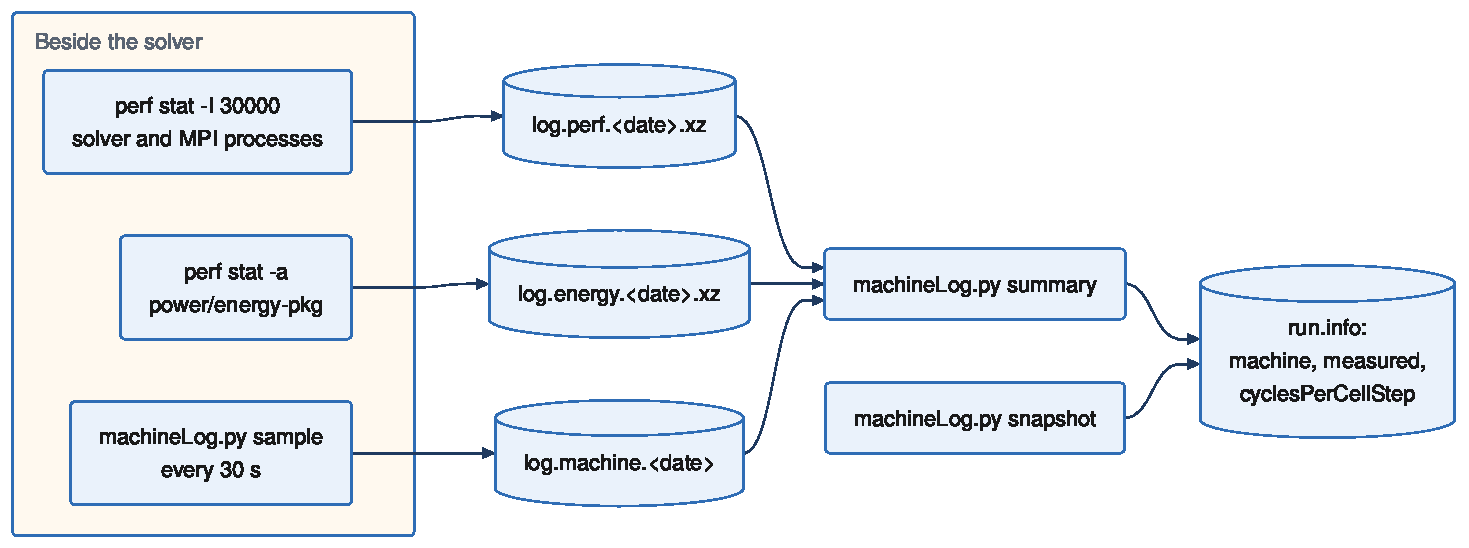
\includegraphics[width=\linewidth]{figures/pdf/measurement.pdf}
  \caption{Measurement during the solver and its record in \texttt{run.info}.}
  \label{fig:measurement}
\end{figure}

\begin{tabularx}{\linewidth}{@{}P{0.26\linewidth} P{0.26\linewidth} L@{}}
\toprule
File & Tool & Contents \\
\midrule
\file{log.perf} & \cmd{perf stat -I 30000} on the solver & Every \unit{30}{s}: task clock, cycles, instructions, front-end stalls, cache misses, migrations, context switches. \\
\file{log.machine} & \file{machineLog.py sample} & Every \unit{30}{s}: wall, monotonic and boot clocks, CPU frequency, load, temperatures of CPU, memory and NVMe, fans, CPU profile. \\
\file{log.energy} & \cmd{perf stat -a -e power/energy-pkg/} & Energy of the CPU package every \unit{30}{s}. Only if \cmd{perf} can count on the whole system. \\
\bottomrule
\end{tabularx}

\begin{longtable}{@{}P{0.32\linewidth} P{0.62\linewidth}@{}}
\caption{Block \texttt{measured} of \texttt{run.info}.}\label{tab:measured}\\
\toprule
Entry & Meaning \\
\midrule
\endfirsthead
\toprule
Entry & Meaning \\
\midrule
\endhead
\ent{suspendedSeconds} & Change of the boot clock minus change of the monotonic clock: the time that the computer was suspended. If it is not 0, the wall time is not a cost. \\
\ent{mhzMean}, \ent{mhzMinOfMean} & Mean clock of all logical CPUs, and the lowest mean of \unit{30}{s}. \\
\ent{tCpuMax}, \ent{tDimm<i>Max}, \ent{tNvmeMax} & Highest temperatures. DDR5 memory doubles its refresh above \unit{85}{\textdegree C}. \\
\ent{profiles} & The CPU profiles during the run. If it is not only \val{performance}, the run does not compare. \\
\ent{cpuSeconds} & CPU time of all solver processes. \\
\ent{cycles}, \ent{instructions} & Totals of all processes. \\
\ent{GHzEffective} & $\text{cycles}/\text{cpuSeconds}$: the real clock of the solver, with turbo and throttling. \\
\ent{IPC} & $\text{instructions}/\text{cycles}$. Low ($\lesssim 1$) in a code that the memory bandwidth limits. \\
\ent{frontendStallFraction} & Cycles with a stopped front end, divided by the cycles. \\
\ent{cacheMisses}, \ent{cpuMigrations}, \ent{contextSwitches} & Indicators of noise. Many migrations show a binding that does not work. \\
\ent{energyPkgJ} & Energy of the CPU package during the solver. \\
\bottomrule
\end{longtable}

The block \ent{machine} gives the state at the start: kernel, sockets, cores, threads
for each core, memory, CPU governor and energy preference, boost, maximum frequency,
CPU profile, fan level, \ent{perf_event_paranoid}, OpenFOAM build and Open MPI version.

\ent{cyclesPerCellStep} is the cost that does not depend on the clock. It includes the
start (the solver reads the mesh), which is small in a run of thousands of steps.

\subsection{Requirements}

\begin{itemize}
\item \ent{kernel.perf_event_paranoid} $\leq 1$ to count the cycles. If not,
  \file{Allrun} shows a message with \val{!!} and runs without \ent{cycles}.
\item $\leq 0$ (or \ent{CAP_PERFMON}) to measure the energy (\cref{sec:prepare-computer}).
\end{itemize}

\subsection{Procedure to get a comparable cost}

\begin{steps}
\item Do the steps of \cref{sec:prepare-computer}.
\item Run one case at a time, with nothing heavy beside it.
\item Use the same number of processes and the same binding for the two solvers: one
  process for each physical core.
\item Before you use the cost of a run, examine \ent{suspendedSeconds},
  \ent{profiles}, \ent{GHzEffective} and \ent{cpuMigrations}.
\end{steps}

\subsection{Do not divide by the clock frequency}

A correction of the wall time by the clock supposes that the time changes as $1/f$.
This is true for a code that the computation limits, not for a code that the memory
bandwidth limits. The two solvers differ in this property: OpenFOAM (low order)
depends more on the memory bandwidth, Nektar++ at a high polynomial order more on the
clock. To measure it, run the same short case at several clock limits
(\ent{scaling_max_freq} at 2, 3 and \unit{4}{GHz}) and fit
\[
  t(f) = t_\text{mem} + \frac{C}{f}.
\]
This procedure is not automated.

\subsection{Runs without this measurement}

The runs before 2026-10-17 have only \file{timeInfo.dat}. An interval with wall time
much larger than CPU time is a suspension. An interval with CPU time much above the
median is a low clock or a load beside the run. Without those intervals, the $h0$ runs
on \texttt{nemepad} cost 20 to 22 core-\textmu s for each cell and step.

\section{Monitor a run}\label{sec:monitor}

\begin{shell}
./post/monitor.sh <run-dir> [seconds]     # default 30 s
\end{shell}

The script plots $C_D$ and $C_L$ against the iteration and the initial residuals on a
logarithmic scale, and draws them again every \val{[seconds]}. It joins the
directories of a continued run. Without a display, it writes
\file{<run-dir>/monitor.png}. It needs \cmd{gnuplot}.

\section{Table of a sweep}\label{sec:sweeptable}

\begin{shell}
./post/sweepTable.sh [runs-dir] > sweep.csv    # default ~/runs
\end{shell}

One line for each run. A run that did not start has empty fields.

\begin{longtable}{@{}P{0.42\linewidth} P{0.52\linewidth}@{}}
\toprule
Columns & Source \\
\midrule
\endhead
\val{case}, \val{mesh}, \val{nCells} & \file{run.info} \\
\val{solver} & \ent{application} in \file{controlDict} \\
\val{Minf}, \val{pInf}, \val{Tinf}, \val{alpha} & \file{flowConditions} \\
\val{status}, \val{steps}, \val{tEnd}, \val{wallSeconds} & Last record of \file{run.info} \\
\val{Cd}, \val{Cl}, \val{CmPitch} & Last line of \file{coefficient.dat} \\
\val{window}, \val{CdMean}, \val{ClMean}, \val{CmPitchMean} & Mean over the window of the stop criterion \\
\val{resUx} \ldots{} \val{resOmega} & Last initial residuals. \val{resP} is empty for \cmd{rhoCentralFoam}. \\
\val{yPlusMin}, \val{yPlusMax}, \val{yPlusAvgWalls}, \val{yPlusAvgFins} & \yplus{} at the last time \\
\bottomrule
\end{longtable}

With a continued run, the coefficients and residuals come from the last start-time
directory only.

\section{Disk}

\begin{itemize}
\item The solver log is compressed with \cmd{xz} at the end. While the solver runs,
  the log grows by 1 to \unit{2}{kB} for each step.
\item \ent{residuals} and the coefficients write one line every 50 steps.
\item \file{constant/polyMesh} is a link to the mesh, except with \ent{--refine}.
\item \ent{purgeWrite 1} keeps only the last time. \file{processor*} is removed when
  \cmd{reconstructPar} ends correctly.
\end{itemize}

\begin{caution}
Many cases link to one mesh. If you remove or make a mesh again, all the cases that
use it lose their mesh.
\end{caution}

\section{Notification}\label{sec:notify}

\file{Allrun} sends a POST request at the end of each run, with the case name,
\val{ok} or \val{failed}, the time, $C_D$ and the hours of wall time. With ntfy, write
the URL of a topic in a file:

\begin{shell}
echo https://ntfy.sh/<topic> > ~/.config/aconcagua/notify
\end{shell}

The topic is public for each person who knows its name: use a name that is difficult
to guess. The environment variable \cmd{NOTIFY_URL} has priority over the file. No
notification comes if \file{runCase.sh} is stopped or if the computer stops.

\chapter{Comparison with Nektar++}\label{ch:nektar}

The aim is to run all the Aconcagua cases with OpenFOAM and with Nektar++ and to
compare the two solvers. Nektar++ adds $p$-refinement to the $h$-refinement of the
meshes, so it has more cases.

``The same case'' is the same mesh, the same free stream and the same initial field.
The schemes, the time integration, the compressible formulation and the turbulence
treatment can differ, but they must be as near as possible. This chapter gives what
each OpenFOAM run records for the Nektar++ run, and what to measure in the same way in
the two solvers.

\section{What must be the same}\label{sec:nektar-same}

\begin{longtable}{@{}P{0.18\linewidth} P{0.34\linewidth} P{0.40\linewidth}@{}}
\caption{Items that the Nektar++ run must reproduce.}\label{tab:nektar-same}\\
\toprule
Item & Where it is & Note \\
\midrule
\endfirsthead
\toprule
Item & Where it is & Note \\
\midrule
\endhead
Mesh & \ent{meshHash} in \file{run.info}; \file{<mesh-dir>/meshHash} & sha256 (16 characters) of \file{points}, \file{faces}, \file{owner}, \file{neighbour}, \file{boundary}. With \ent{--refine}, the hash of the refined mesh. The Nektar++ mesh comes from the same \file{polyMesh}. \\
Half mesh & \file{meshInfo}: \ent{sector half} & Symmetry plane $z = 0$. \ent{Aref} is half the frontal area. \\
Free stream & block \ent{flow} in \file{run.info} & \ent{Minf}, \ent{alpha}, \ent{pInf}, \ent{Tinf}, \ent{Uinf}, \ent{rhoInf}, \ent{muInf}, the components of $\mathbf{U}$. \\
Reynolds number & \ent{RePerMetre}, \ent{ReD}, \ent{ReL} & From \ent{rhoInf}, \ent{Uinf} and \ent{muInf}, on the diameter and on the body length. \\
Gas & \ent{Rgas}, \ent{gammaGas}, \ent{Cp}, \ent{RgasThermo} & $R$ is 287.05 in \file{flowDerived} and 287.10 in the thermophysical model (\cref{sec:thermo}). \\
Viscosity & \ent{sutherland (As Ts)} & $\mu = A_s\sqrt{T}/(1 + T_s/T)$. \\
Conductivity & \ent{PrEucken} & $Pr = 0.690$ from the Eucken correction, not 0.72. Nektar++ must use this value. \\
Turbulence & \ent{turbulence}, \ent{Prt}, \ent{Ti}, \ent{nuRatio}, \ent{kInlet}, \ent{omegaInlet} & $k$--$\omega$ SST with \ent{nutUSpaldingWallFunction}. \\
Wall & \ent{wallT}, \ent{wallNut} & Adiabatic (\val{zeroGradient} on $T$), no slip. \\
Initial field & \ent{initial} & \val{uniform free stream}, or the run that was mapped. \\
References & \file{FOcommon} & \ent{CofR (0 0 0)} (nose tip); drag and lift in wind axes; \ent{lRef}; \ent{Aref}. \\
\bottomrule
\end{longtable}

\section{What to compare}

\begin{tabularx}{\linewidth}{@{}P{0.32\linewidth} L@{}}
\toprule
Quantity & OpenFOAM file \\
\midrule
History of $C_D$, $C_L$, $C_m$ & \file{forceCoeffs1/*/coefficient.dat}, every 50 steps \\
Pressure and viscous force & \file{forces1/*/force.dat} \\
$C_p$, $\tau_w$, \yplus{} along the body & \file{samples/*/skinZ0_*.csv}, \file{skinY0_*.csv} \\
Wake profiles & \file{samples/*/wake05}, \file{wake1}, \file{wake2}, \file{wake5} \\
Axis and free-stream check & \file{samples/*/axis_*.csv}, \file{freeStream_*.csv} \\
Skin and symmetry plane & \file{surfaces/*/} (VTK) \\
Cost & \ent{cyclesPerCellStep}, \ent{cpuSeconds}, \ent{energyPkgJ}, \ent{GHzEffective} in \file{run.info} \\
\bottomrule
\end{tabularx}

\section{How to measure in the same way}

\begin{itemize}
\item \textbf{Degrees of freedom.} OpenFOAM: $N_\text{cells}$ for each variable.
  Nektar++: $N_\text{elements}\,(P+1)^3$ for each variable on hexahedra (a different
  count on prisms and tetrahedra). Compare the cost for each degree of freedom and
  each step, in cycles.
\item \textbf{Convergence.} Each solver stops with its own criterion and its own
  step. For the cost to the result, apply one criterion to the two histories of $C_D$,
  against the accumulated cost. Do not use the residuals: each code normalizes them
  differently.
\item \textbf{Refinement.} Each pair $(h, P)$ of Nektar++ is a case. The cost for each
  degree of freedom puts them on the same curve as $h1$ to $h3$ of OpenFOAM.
\item \textbf{Computer.} Use the procedure of \cref{sec:measurement}, the same
  computer, the same number of processes and the same binding. Do not divide by the
  clock frequency: measure the dependence on the clock.
\end{itemize}

\chapter{Flight data}\label{ch:flight}

The TeleMega recorded the IREC flight in Midland. \file{flightData/cdFlight.py}
calculates from these data the atmosphere of that day, the speed, the drag
coefficient in the coast phase and the conditions of the sweep. It plots the result
against the CFD runs and OpenRocket.

\section{Command}

\begin{shell}
python3 flightData/cdFlight.py [--csv AconcaguaIREC_TeleMega.csv] [--mass 24.52]
        [--runs ~/runs] [--ork rocket.ork] [--alphas 0,8] [--out cdFlight.png]
\end{shell}

\begin{tabularx}{\linewidth}{@{}P{0.24\linewidth} P{0.26\linewidth} L@{}}
\toprule
Option & Default & Function \\
\midrule
\ent{--csv} & \file{flightData/AconcaguaIREC_TeleMega.csv} & TeleMega data. \\
\ent{--mass} & \unit{24.52}{kg} & Mass after burnout, from the OpenRocket simulation. \\
\ent{--runs} & \file{~/runs} & Runs to plot. The script uses the last segment of each run. \\
\ent{--ork} & \file{~/Downloads/207 - Aconcagua.ork} & OpenRocket file for its $C_D$ curve. Optional. \\
\ent{--alphas} & \val{0,8} & Angles of the runs to plot. \\
\ent{--tanchor} & \unit{18}{s} & Time of the speed anchor. \\
\ent{--out} & \file{flightData/cdFlight.png} & Plot. \\
\bottomrule
\end{tabularx}

\section{Method}

\Cref{fig:flight-method} shows the method. All values come from the telemetry,
except the mass.

\begin{figure}[htbp]
  \centering
  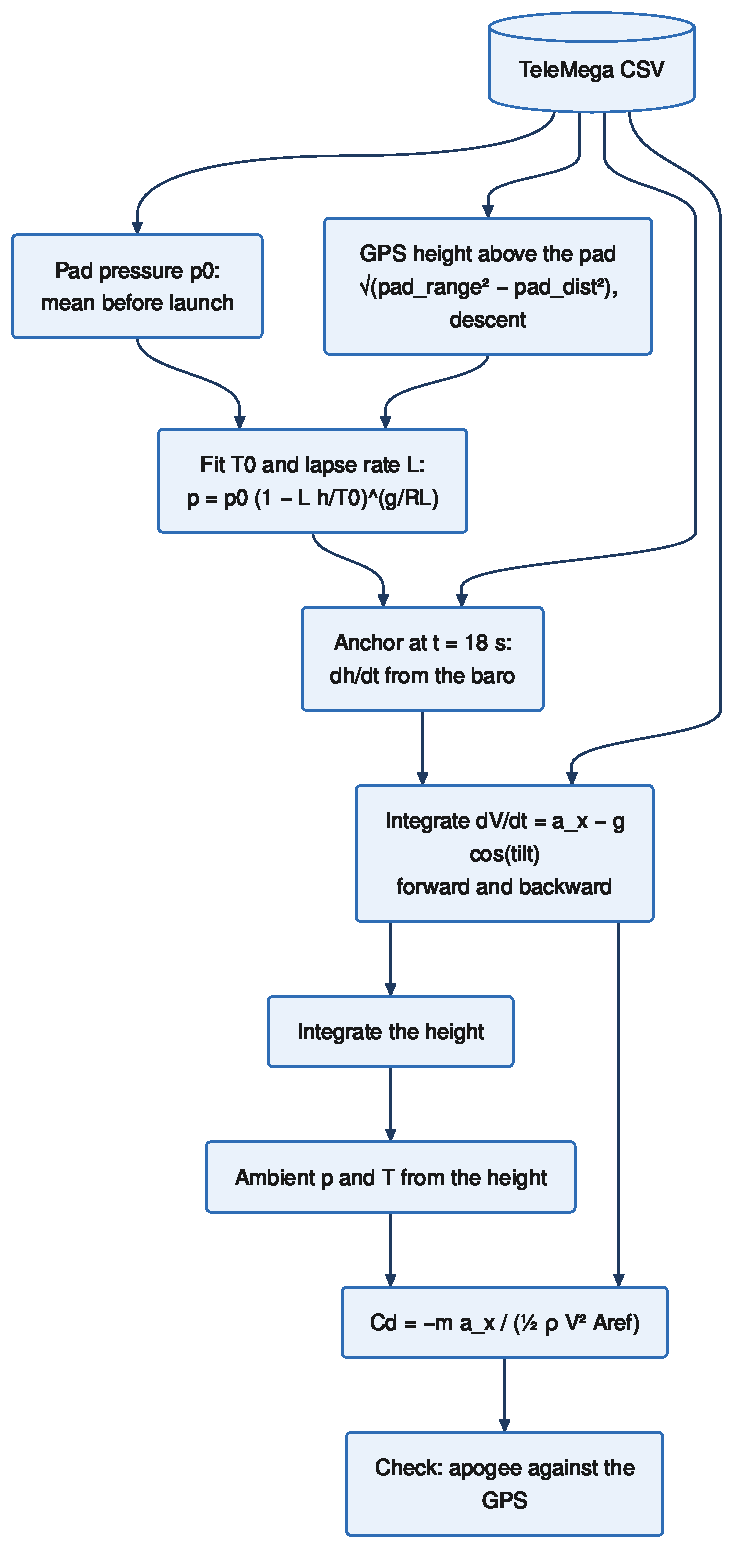
\includegraphics[height=0.5\textheight]{figures/pdf/flight.pdf}
  \caption{Calculation of the flight drag coefficient.}
  \label{fig:flight-method}
\end{figure}

\begin{steps}
\item \textbf{Atmosphere.} The pad pressure $p_0$ is the mean before launch. During
  the descent, the GPS gives the height above the pad,
  $h = \sqrt{\texttt{pad\_range}^2 - \texttt{pad\_dist}^2}$, and the barometer gives
  the pressure without shocks. The script fits $T_0$ and the lapse rate $L$ in
  \[
    p = p_0\left(1 - \frac{L\,h}{T_0}\right)^{g/(R L)}.
  \]
  Result: $p_0 = \unit{90\,565}{Pa}$, $T_0 = \unit{305.0}{K}$,
  $L = \unit{7.2}{K/km}$, from 215 GPS points, with an rms error of 0.3\,\% in
  $\ln p$. The air was approximately \unit{20}{K} warmer than the ISA at all heights.
\item \textbf{Speed.} The script does not use the column \texttt{speed} of the
  TeleMega: its filter converts pressure to height with the ISA, and it gives
  approximately 10\,\% less in the coast. Above $M \approx 0.8$ the barometer is not
  used either, because the static ports are behind shocks. The script integrates the
  axial accelerometer, forward and backward from $t = \unit{18}{s}$:
  \[
    \frac{dV}{dt} = a_x - g\cos\theta_\text{tilt}.
  \]
  At $t = \unit{18}{s}$ ($M \approx 0.65$) the speed comes from the derivative of the
  barometric height with the fitted atmosphere.
\item \textbf{Height and ambient state.} The script integrates $V\cos\theta$ for the
  height, and calculates $p$ and $T$ from the height with the fitted atmosphere.
\item \textbf{Drag.} In the coast, $a_x$ is the axial specific force, so
  $D = -m\,a_x$ and
  \[
    C_D = \frac{-m\,a_x}{\tfrac12\rho V^2 A_\text{ref}}, \qquad
    A_\text{ref} = \pi\,(\unit{0.0755}{m})^2.
  \]
  The script uses the data from $t = \unit{4.0}{s}$, when the residual thrust ends.
\item \textbf{Check.} The integrated apogee is \unit{8137}{m} above the pad. The GPS
  gives \unit{8083}{m} (0.7\,\% difference).
\end{steps}

\section{Results}

\begin{figure}[htbp]
  \centering
  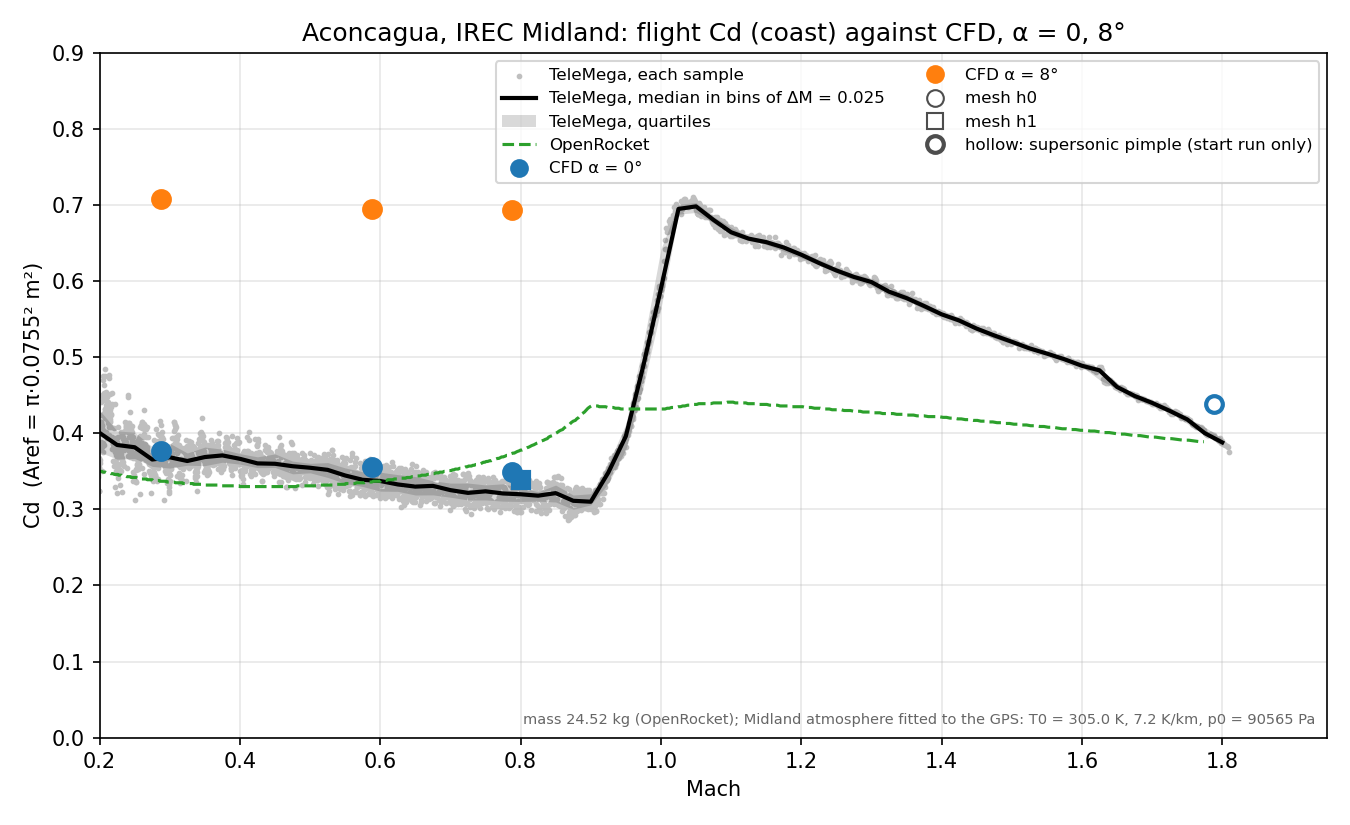
\includegraphics[width=\linewidth]{../../flightData/cdFlight.png}
  \caption{$C_D$ of the flight (coast) against the runs of the first sweep (ISA conditions, \texttt{\textasciitilde/runs.sin-medicion}) and OpenRocket.}
  \label{fig:cdflight}
\end{figure}

\begin{table}[htbp]
\centering
\caption{$C_D$ of the flight and of the CFD at $\alpha = 0$ (first sweep, ISA conditions, 2026-10-17).}\label{tab:cd-flight}
\begin{tabular}{@{}ccccc@{}}
\toprule
$M$ & Flight & CFD & CFD/flight & OpenRocket \\
\midrule
0.3 & 0.369 & 0.376 ($h0$) & 1.02 & 0.336 \\
0.6 & 0.337 & 0.356 ($h0$) & 1.05 & 0.337 \\
0.8 & 0.320 & 0.349 ($h0$), 0.339 ($h1$) & 1.09, 1.06 & 0.378 \\
$\approx$1.03 & $\approx$0.70 (peak) & -- & -- & $\approx$0.44 \\
1.2 & $\approx$0.64 & -- & -- & $\approx$0.43 \\
1.8 & 0.388 & 0.438 (pimple start only) & 1.13 & 0.389 \\
\bottomrule
\end{tabular}
\end{table}

\begin{itemize}
\item From $M = 0.3$ to $0.8$ the CFD is 2 to 9\,\% above the flight, and it decreases
  from $h0$ to $h1$.
\item In the flight, $C_D$ doubles from $M = 0.9$ to $1.0$. OpenRocket does not show
  this peak. No CFD run is in this range yet.
\item The flight value at $M = 1.8$ is 13\,\% below the pimple start run. That run is
  not a result of the central template.
\end{itemize}

\section{Angle of attack in the flight}\label{sec:flight-alpha}

The rocket rolls at approximately 4 revolutions per second in the coast. The mean
lateral acceleration follows the square of the roll rate with a constant radius of
approximately \unit{2.8}{cm}: it is the centripetal acceleration of a sensor off the
axis. An aerodynamic normal force has a fixed direction in space, so in the body axes
it turns with the roll. The oscillation of the lateral acceleration at the roll
frequency gives $C_N \approx 0.01$ to $0.03$. With $C_{N\alpha} \approx \unit{18}{/rad}$
from the CFD, $\alpha < 0.2^\circ$ in all the coast. The sensor noise is in this value,
so it is an upper limit.

\section{Uncertainty}

\begin{tabularx}{\linewidth}{@{}P{0.24\linewidth} L@{}}
\toprule
Source & Effect \\
\midrule
Mass & $C_D$ is proportional to the mass, which is a design value of OpenRocket, not a measurement. \\
Wind & No data. The speed is relative to the ground. \\
Flight path & The gravity term uses the attitude as the direction of the flight path. With $\alpha < 0.2^\circ$ the error is small. \\
Atmosphere & The fit gives one lapse rate from the pad to \unit{8}{km}. The local layers differ from the fit by up to \unit{7}{K}. \\
\bottomrule
\end{tabularx}

\chapter{Validation}\label{ch:validation}

Do the procedures in this sequence: the checks on each run, the subsonic references,
the transonic and supersonic references, the flight, and the mesh convergence before you
publish a value.

\section{Checks on each run}\label{sec:run-checks}

\begin{longtable}{@{}P{0.24\linewidth} P{0.32\linewidth} P{0.36\linewidth}@{}}
\caption{Checks on each run.}\label{tab:run-checks}\\
\toprule
Check & Correct result & Cause if not correct \\
\midrule
\endfirsthead
\toprule
Check & Correct result & Cause if not correct \\
\midrule
\endhead
$C_L$, $C_m$ at $\alpha = 0$; $C_l$ (roll) & $\approx 0$ & The mesh is not symmetric, or the run did not converge. \\
\yplus{} on each wall patch & Near the estimate of \cref{sec:layers}, and equal on the meshes of a study & The first cell changed. \\
Minimum and maximum of $T$ & Physical: at most near the stagnation temperature & The start transient is not resolved. \\
Iterations & More than \ent{minIter}, and the criterion met & The run stopped before it was steady. \\
$C_N(\alpha)$ & Linear at small $\alpha$ & The run did not converge, or the fins are not resolved. \\
Machine record & No suspension; one CPU profile & The cost is not usable (\cref{sec:measurement}). \\
\bottomrule
\end{longtable}

\section{Subsonic flow: Barrowman}\label{sec:barrowman}

The slender-body equations of \citet{barrowman1967,barrowman1966}, which OpenRocket
uses, give the normal force and the centre of pressure of each component, referred to
the body cross-section and for each radian. \citet[ch.~2]{fleeman2012} gives equivalent
equations for the fins and the fin-body interference.

\begin{tabularx}{\linewidth}{@{}l L@{}}
\toprule
Component & $C_{N\alpha}$ \\
\midrule
Nose & 2, for any nose of revolution \\
Cylinder & $\approx 0$ \\
Boattail & $2\left[(d_\text{base}/d)^2 - 1\right]$ \\
Fins, $N$ fins & $K_{fb}\,\dfrac{4N(s/d)^2}{1 + \sqrt{1 + \left(\dfrac{2 l_m}{c_r + c_t}\right)^2}}$, \quad $K_{fb} = 1 + \dfrac{r}{s + r}$ \\
\bottomrule
\end{tabularx}

\medskip
$s$ is the exposed semi-span, $c_r$ and $c_t$ the root and tip chords, $l_m$ the length
of the mid-chord line, $r$ the body radius.

\begin{steps}
\item Run an angle-of-attack sweep at small angles.
\item Calculate the slope of $C_N = C_L\cos\alpha + C_D\sin\alpha$ against $\alpha$ in
  radians. $C_L$ is normal to the free stream, $C_N$ to the body axis.
\item Compare the slope with the sum of the components. For the breakdown, add one
  \ent{forceCoeffs} function object for each patch.
\end{steps}

\paragraph{Drag at zero angle.} Compare the components, not only the total. The
viscous part of \file{force.dat} against the skin friction $C_f S_\text{wet}/A_\text{ref}$
with $C_f = 0.0576\,Re_L^{-1/5}$ \citep[ch.~21]{schlichting1979} and the form factors
$1 + 1/(2L/d)$ (body) and $1 + 2t/c$ (fins); the base drag against
\citet[ch.~3]{hoerner1965}. $Re_L$ of each case is in \file{run.info}.

\section{Transonic and supersonic flow}\label{sec:supersonic-validation}

\begin{enumerate}
\item \textbf{Tutorial of the template.} Run the \cmd{rhoCentralFoam} tutorial
  \file{biconic25-55Run35} and compare it with its published data. This separates a
  configuration error from a mesh error.
\item \textbf{Oblique shock on a wedge.} The $\theta$--$\beta$--$M$ relation is exact
  \citep[ch.~4]{anderson2003}:
  \[
    \tan\theta = 2\cot\beta\,\frac{M^2\sin^2\beta - 1}{M^2(\gamma + \cos 2\beta) + 2}.
  \]
  The tutorial \file{wedge15Ma5} is this case.
\item \textbf{Flight.} \Cref{ch:flight}. The CFD must show the transonic drag rise
  of the flight. If it does not, the mesh is too coarse where the shocks occur.
\item \textbf{OpenRocket.} Semi-empirical: it finds gross errors, not small ones.
\end{enumerate}

\section{Mesh convergence}\label{sec:gci}

With $f_1$, $f_2$, $f_3$ the results on the fine, medium and coarse meshes, the
representative cell size $h = N^{-1/3}$ and the ratio $r = h_\text{coarse}/h_\text{fine}$,
the method of \citet{celik2008} gives the observed order $p$, the extrapolated value and
the grid convergence index:
\[
  p = \frac{\ln\left[(f_3 - f_2)/(f_2 - f_1)\right]}{\ln r},\qquad
  f_\text{ext} = f_1 + \frac{f_1 - f_2}{r^p - 1},\qquad
  \text{GCI}_{12} = 1.25\,\frac{|(f_1 - f_2)/f_1|}{r^p - 1}.
\]
With unequal ratios, use the iterative form of \citet{celik2008}. If
$(f_3 - f_2)/(f_2 - f_1) < 0$, the convergence is oscillatory and the equations do not
apply \citep{roache1994}.

\section{Record}

For each published value keep: \file{meshDict}, \file{meshInfo} and
\file{log.checkMesh} of the mesh; the STL file or its commit; \file{run.info},
\file{flowConditions} and \file{config.json} of the run; and \file{postProcessing/}.
With these files another person can make the result again.

\chapter{Troubleshooting}\label{ch:troubleshooting}

\begin{longtable}{@{}P{0.30\linewidth} P{0.30\linewidth} P{0.32\linewidth}@{}}
\caption{Symptoms, causes and remedies.}\label{tab:troubleshooting}\\
\toprule
Symptom & Cause & Remedy \\
\midrule
\endfirsthead
\toprule
Symptom & Cause & Remedy \\
\midrule
\endhead
\val{source the OpenFOAM bashrc first} & No OpenFOAM environment. & \Cref{ch:setup}. \\
Negative cell volumes. & The surface breaks a rule of \cref{tab:surface-rules}, or a level is too coarse for a curvature. & Do not use the mesh. Correct the surface or the levels. \\
A wall patch without layers. & No entry in \ent{patchBoundaryLayers}. & \Cref{sec:layers}. \\
Incorrect domain, or a number with a decimal comma. & \cmd{awk} in a locale with a decimal comma. & \Cref{sec:ts-locale}. \\
\cmd{rhoCentralFoam} fails in the first iterations. & Start from a uniform free stream. & \Cref{sec:supersonic-start}. \\
Courant number of order $10^7$ in the log. & Normal with \ent{localEuler}. & \Cref{sec:ts-courant}. \\
A run with \ent{--init} behaves as a start from rest. & \cmd{mapFields} failed. & \Cref{sec:ts-mapfields}. \\
\cmd{taskset} shows all CPUs for a process; many migrations. & The binding does not work. & \Cref{sec:binding}. \\
Wall time much larger than CPU time; \ent{suspendedSeconds} $> 0$. & The computer suspended. & \Cref{sec:prepare-computer}. The coefficients are correct; the cost is not. \\
\ent{profiles} has more than one value; low \ent{GHzEffective}. & The CPU profile changed during the run. & \Cref{sec:prepare-computer}. \\
No \ent{cycles} in \file{run.info}. & \ent{perf_event_paranoid} too high. & \Cref{sec:prepare-computer}. \\
The computer swaps or the run stops for memory. & The mesh is too large for the memory. & Scale the memory from a coarser mesh (\cref{tab:requirements}). \\
\cmd{pkill -f} stops your own shell. & The command line contains the pattern. & Stop the process by its number. \\
A sweep reads wrong lines. & The sweep file was edited while it ran. & Stop, edit, start again. \\
A script does unexpected things after an edit. & \cmd{sh} reads a script while it runs it. & Do not edit a script that runs. \\
A dictionary does not parse near its banner. & \texttt{*/} in the banner comment closes the comment. & Remove \texttt{*/}. \\
A script continues after a failed application. & \cmd{runApplication} returns 0 on \val{FOAM FATAL ERROR}. & Read each log, as \file{Allmesh} and \file{Allrun} do. \\
\bottomrule
\end{longtable}

\section{mapFields on the same mesh}\label{sec:ts-mapfields}

\cmd{mapFields} can stop with a segmentation fault when the source and the target are
the same mesh. Between different meshes it works. \file{Allrun} stops the run if the
log of \cmd{mapFields} or \cmd{changeDictionary} does not end with \val{End}; a check
for \val{FOAM FATAL} only does not detect a segmentation fault. On the same mesh, a copy
of the fields of the source run is an alternative that does not interpolate.

\section{The Courant number with a local time step}\label{sec:ts-courant}

With \ent{localEuler}, \cmd{rhoCentralFoam} calculates the Courant number with the
global \ent{deltaT}, so the value in the log is meaningless. Read
\val{Flow time scale min/max} (\cref{sec:lts}).

\section{Decimal comma}\label{sec:ts-locale}

In a locale with a decimal comma, \cmd{awk} reads and writes numbers with a comma, and
OpenFOAM reads them incorrectly. Each script that calculates with \cmd{awk} sets
\cmd{LC_ALL=C}. Do the same in a new script.

\section{Rules for a change to the scripts}

\begin{itemize}
\item Measure before you propose a change; a change without a number is not complete.
\item Do not put a Python script in a bash here-document: a \texttt{\textbackslash n}
  in an f-string becomes a real new line and breaks the file.
\item After a change, run one short case and examine \file{run.info}.
\item Change this guide in the same commit.
\end{itemize}


\appendix
\crefalias{chapter}{appendix}
\chapter{Quick reference}\label{app:quickref}

\section{Commands}

\begin{shell}
source /usr/lib/openfoam/openfoam2412/etc/bashrc

# geometry and one mesh
python3 mesh/makeRocket.py mesh/stl/Aconcagua_biconvex117_roll45.stl --finRoll 45
mesh/Allmesh ~/meshes/h1 --maxCellSize 1.6 --nLayers 10 --thicknessRatio 1.2
./post/firstLayer.py ~/meshes/h1

# one case
./newCase.sh ~/runs/test --mesh ~/meshes/h1 --solver pimple --Minf 0.8 --np 8
cd ~/runs/test && ./Allrun 8

# sweep
./runMesh.sh meshes.txt ~/meshes
nohup ./runCase.sh sweepSubsonic.nemepad.txt > ~/log.sweepSubsonic.nemepad 2>&1 &

# results
./post/monitor.sh ~/runs/test
./post/sweepTable.sh ~/runs > sweep.csv
python3 flightData/cdFlight.py

# check the binding and the measurement of a running case
for p in $(pgrep -x rhoPimpleFoam); do taskset -cp $p; done
tail -3 ~/runs/<case>/log.machine
\end{shell}

\section{Run names}

\texttt{m<M>-a<alpha>-h<n>[-pimple]}: \texttt{m08} is $M = 0.8$, \texttt{a04} is
$\alpha = 4^\circ$, \texttt{h1} is the mesh. The suffix \texttt{-pimple} marks the
\cmd{rhoPimpleFoam} start run of a supersonic chain.

\section{Key values}

\begin{tabularx}{\linewidth}{@{}P{0.42\linewidth} L@{}}
\toprule
Item & Value \\
\midrule
Reference area, full rocket & $A_\text{ref} = \pi\,(0.0755)^2 = \unit{0.0179081}{m\textsuperscript{2}}$ \\
Reference length & $l_\text{ref} = d = \unit{0.151}{m}$ \\
Moment reference & Nose tip, $(0, 0, 0)$ \\
Rocket length & \unit{2.955}{m} \\
First cell on the body & $t_1 \approx \unit{0.10}{mm}$, $y \approx \unit{0.05}{mm}$ \\
Stop criterion & $|\overline{C_D} - C_D| < 0.007$ over 1000 iterations \\
Memory & approximately \unit{3}{GB} for each million cells \\
Midland atmosphere & $p_0 = \unit{90\,565}{Pa}$ at \unit{896}{m} MSL, $T_0 = \unit{305.0}{K}$, \unit{7.2}{K/km} \\
\bottomrule
\end{tabularx}

\chapter{Glossary}\label{app:glossary}

\section{Terms and abbreviations}

\begin{longtable}{@{}P{0.24\linewidth} P{0.70\linewidth}@{}}
\toprule
Term & Definition \\
\midrule
\endhead
Binding & The assignment of each MPI process to fixed CPU cores. \\
Boattail & The cone at the rear of the body, from the body diameter to the base. \\
Chain & A sequence of runs at one flight condition, each started from the run on the coarser mesh. \\
Coast & The flight phase after the motor burnout, $t > \unit{4}{s}$. \\
CFD & Computational fluid dynamics. \\
DOF & Degree of freedom: one unknown of the discrete system. \\
GCI & Grid convergence index \citep{celik2008}. \\
IPC & Instructions per cycle. \\
ISA & International Standard Atmosphere. \\
LTS & Local time stepping (\ent{localEuler}). \\
Mesh $h0$ to $h3$ & The meshes of the sweep (\cref{tab:meshes}). \\
MSL & Mean sea level. \\
RANS & Reynolds-averaged Navier--Stokes equations. \\
Run & One case directory and its executions. \\
SST & Shear-stress transport ($k$--$\omega$ SST model). \\
Sweep & A file with one run on each line, and its execution by \file{runCase.sh}. \\
Template & \file{case-central/} or \file{case-pimple/}: the files from which \file{newCase.sh} makes a case. \\
TVD & Total variation diminishing. \\
$y^+$ & Distance of the first cell centre from the wall, in wall units: $y\,u_\tau/\nu$. \\
\bottomrule
\end{longtable}

\section{Symbols}

\begin{longtable}{@{}P{0.24\linewidth} P{0.50\linewidth} P{0.18\linewidth}@{}}
\toprule
Symbol & Definition & Unit \\
\midrule
\endhead
$A_\text{ref}$ & Reference area & m\textsuperscript{2} \\
$a$ & Speed of sound & m/s \\
$C_D$, $C_L$, $C_N$ & Drag, lift and normal-force coefficients & -- \\
$C_m$ & Pitching-moment coefficient about the nose tip & -- \\
$C_p$ & Pressure coefficient & -- \\
$c_p$, $c_v$ & Specific heats & J/(kg\,K) \\
$d$ & Body diameter & m \\
$k$, $\omega$ & Turbulent kinetic energy, specific dissipation rate & m\textsuperscript{2}/s\textsuperscript{2}, 1/s \\
$M$ & Mach number & -- \\
$p$, $T$, $\rho$ & Pressure, temperature, density & Pa, K, kg/m\textsuperscript{3} \\
$Pr$, $Pr_t$ & Laminar and turbulent Prandtl numbers & -- \\
$R$ & Gas constant of air & J/(kg\,K) \\
$Re$ & Reynolds number & -- \\
$t_1$ & Thickness of the first wall cell & m \\
$\alpha$, $\beta$ & Angle of attack, angle of sideslip & deg \\
$\gamma$ & Ratio of specific heats & -- \\
$\mu$, $\nu$, $\nu_t$ & Dynamic, kinematic and eddy viscosity & Pa\,s, m\textsuperscript{2}/s \\
$\tau_w$ & Wall shear stress & Pa \\
\bottomrule
\end{longtable}


\bibliographystyle{unsrtnat}
\bibliography{references}

\end{document}
